% Department of Mathematics, Bilkent University
% Emre Sen

\documentclass[12pt]{amsart}
\usepackage{amsmath,amssymb}
\usepackage{eufrak}
\usepackage{amsthm}
\usepackage{enumitem}
\usepackage{setspace}
\usepackage{graphicx}
\usepackage{graphics}
\usepackage{color}
\usepackage[dvipsnames]{xcolor}
%\pagecolor{yellow!30}
\usepackage{hyperref}
%\usepackage{array}
\usepackage{youngtab}
\usepackage{xcolor}
\usepackage{enumitem}
\usepackage{yfonts}

%\usepackage{biblatex}


\hypersetup{ colorlinks,
 linkcolor={blue},  citecolor={BrickRed}, urlcolor={blue}}

\usepackage{amsthm,thmtools,xcolor}


\usepackage{marginnote}
\usepackage{lscape}
\usepackage{faktor}
\usepackage{hyperref}
\usepackage[normalem]{ulem}
\usepackage{bm}
\usepackage{afterpage}
%\usepackage{pgfplots}
\usepackage{mathrsfs}
\usepackage[all]{xy}
\xyoption{matrix}
\xyoption{arrow}
\usepackage{tikz}
\usetikzlibrary{calc,shadings,patterns}
\usetikzlibrary{matrix}
\usetikzlibrary{arrows}
\usetikzlibrary{matrix}
\usepackage{verbatim}
\usepackage{multirow}
%\usepackage{geometry}
%\usepackage{tikz-cd}
\usetikzlibrary{decorations.pathreplacing}
% http://ctan.org/pkg/{enumitem,pifont,xcolor}
\usepackage{enumitem,pifont,xcolor}% http://ctan.org/pkg/{enumitem,pifont,xcolor}
\definecolor{myblue}{RGB}{0,29,119}

% The package can be used temporarily only to show the cross-reference labels
%\usepackage{showkeys}
% This paragraph resets the sizes of the printed area of the page
\hoffset -1.5cm
\voffset -1cm
\textwidth 15.5truecm
\textheight 22.5truecm
% This paragraph defines the macros for theorems and the like
%\newtheorem{thm}{Theorem}[subsection]





\newtheorem{theorem}{Theorem}[section]
\newtheorem{proposition}[theorem]{Proposition}
\newtheorem{corollary}[theorem]{Corollary}
\newtheorem{lemma}[theorem]{Lemma}
% This paragraph defines the macros for definitions and the like
\theoremstyle{definition}
\newtheorem{definition}[theorem]{Definition}
\newtheorem{example}[theorem]{Example}
\newtheorem{conjecture}[theorem]{Conjecture}
\newtheorem{remark}[theorem]{Remark}
\newtheorem{remarks}[theorem]{Remarks}
\newtheorem{ideas}[theorem]{Ideas}
\newtheorem{cons}[theorem]{Construction}
\newtheorem{solution}[theorem]{Solution}
\newtheorem{notation}[theorem]{Notation}
\newtheorem{claim}[theorem]{Claim}
\newtheorem{problem}[theorem]{Problem}
\newtheorem{question}[theorem]{Question}
\newtheorem{com}[theorem]{Comments-Citations}
\newtheorem{wa}[theorem]{Warning for writer}
\newtheorem{anal}[theorem]{Analogy}
\newtheorem*{theorem*}{Theorem}
%\newtheorem{corollary}[theorem]{Corollary}





% The following paragraph writes the equation numbers with two counters,
% the first is the section number and the second resets within the section.
\makeatletter
\@addtoreset{equation}{section}
\makeatother
\renewcommand\theequation{\arabic{section}.\arabic{equation}}
% The next paragraph defines macros for special roman letters to be used
\newcommand{\Aa}{{\mathbb A}} % the set of complex numbers
\newcommand{\Cc}{{\mathbb C}} % the set of complex numbers
\newcommand{\Nn}{{\mathbb N}} % the set of natural numbers
\newcommand{\Qq}{{\mathbb Q}} % the set of rational numbers
\newcommand{\Zz}{{\mathbb Z}} % the set of integer numbers
\newcommand{\Dd}{{\mathbb D}} % the unit disk
\newcommand{\Rr}{{\mathbb R}} % the set of real numbers
\newcommand{\Tt}{{\mathbb T}} % the unit circle (the one dimensional torus)
\newcommand{\Hh}{{\mathbb H}} % the set of quaternions
\newcommand{\Pp}{{\mathbb P}} %projectivity symbol
\newcommand{\Ss}{{\mathbb S}} %sphere
%new functions
\DeclareMathOperator{\sign}{sign}
\DeclareMathOperator{\End}{End}
\DeclareMathOperator{\coker}{coker}
\DeclareMathOperator{\im}{Im}
\DeclareMathOperator{\findim}{fin.\! dim}
\DeclareMathOperator{\gordim}{gor.\! dim}
\DeclareMathOperator{\gldim}{gl\,\! dim}
\DeclareMathOperator{\domdim}{dom.\! dim}
\DeclareMathOperator{\codom}{codom.\! dim}
\DeclareMathOperator{\deloop}{del}
\DeclareMathOperator{\indim}{in.\!dim}
\DeclareMathOperator{\Hom}{Hom}
\DeclareMathOperator{\ext}{Ext}
\DeclareMathOperator{\Ext}{Ext}
\DeclareMathOperator{\pdim}{p.\!dim}
\DeclareMathOperator{\rank}{Rank}
\DeclareMathOperator{\add}{add}
\DeclareMathOperator{\soc}{soc}
\DeclareMathOperator{\topp}{top}
\DeclareMathOperator{\modd}{mod-\!}
\DeclareMathOperator{\rad}{rad}
\DeclareMathOperator{\cogen}{CoGen}
\DeclareMathOperator{\defect}{def}
\DeclareMathOperator{\proj}{\mathsf{Proj}}
\DeclareMathOperator{\ideal}{\mathsf{Ideal}}
\DeclareMathOperator{\ind}{\mathsf{ind}}



% The next paragraph defines macros for caligraphic letters
\newcommand{\cA}{{\mathcal A}}
\newcommand{\cB}{{\mathcal B}}
\newcommand{\cC}{{\mathcal C}}
\newcommand{\cD}{{\mathcal D}}
\newcommand{\cE}{{\mathcal E}}
\newcommand{\cF}{{\mathcal F}}
\newcommand{\cG}{{\mathcal G}}
\newcommand{\cH}{{\mathcal H}}
\newcommand{\cI}{{\mathcal I}}
\newcommand{\cJ}{{\mathcal J}}
\newcommand{\cK}{{\mathcal K}}
\newcommand{\cL}{{\mathcal L}}
\newcommand{\cM}{{\mathcal M}}
\newcommand{\cN}{{\mathcal N}}
\newcommand{\cO}{{\mathcal O}}
\newcommand{\cP}{{\mathcal P}}
\newcommand{\cp}{{\mathcal p}}
\newcommand{\cQ}{{\mathcal Q}}
\newcommand{\cq}{{\mathcal q}}
\newcommand{\cR}{{\mathcal R}}
\newcommand{\cS}{{\mathcal S}}
\newcommand{\cT}{{\mathcal T}}
\newcommand{\cU}{{\mathcal U}}
\newcommand{\cV}{{\mathcal V}}
\newcommand{\cX}{{\mathcal X}}
\newcommand{\cY}{{\mathcal Y}}
\newcommand{\cW}{{\mathcal W}}
\newcommand{\cZ}{{\mathcal Z}}
% The next paragraph defines special macros
\newcommand{\iac}{\mathrm{i}} % the imaginary i
\newcommand{\de}{\operatorname{d}} % the differential
\newcommand{\deriv}{\operatorname{D}}
\renewcommand{\theenumi}{\Roman{enumi}}
\renewcommand{\labelenumi}{\theenumi}
\renewcommand{\rank}{\operatorname{rank} }


%\newcommand{\co1}[1]{$\cS^{#1}$}
%\newcommand{\co2}[1]{$\cM^{#1}$}

\newcommand{\co}[1]{\textcolor{red}{#1}}
\newcommand{\ho}[1]{\Hom_{\Lambda}(\cP_\Lambda,{#1})}

\newcommand{\cWW}{\cW(\Gamma'_L)}
\newcommand{\cBB}{\cB(\cW(\Gamma'_L))}


% Authors macros for complicated commands can be used, but be careful!
\providecommand{\AMS}{$\mathcal{A}$\kern-.1667em%
\lower.25em\hbox{$\mathcal{M}$}\kern-.125em$\mathcal{S}$}
% Use of macros should confine the general rules for AMS-LaTeX. It is
% recommended to use \newcommand and \renewcommand instead of the TeX
% primitive \def
% Next is an example of macro I designed for numbering items that are
% different than the available ``itemize, description'' environments.
% You can use it if you want!
\newcommand{\nr}[1]{\vspace{0.1ex}\noindent\hspace*{12mm}\llap{\textup{(#1)}}}
% Topmatter produces the title, author, abstract, etc.
\setcounter{secnumdepth}{6}
\setcounter{tocdepth}{2}

% sayfa genisletme
\def\changemargin#1#2{\list{}{\rightmargin#2\leftmargin#1}\item[]}
\let\endchangemargin=\endlist 



\newtheorem{innercustomthm}{Theorem}
\newenvironment{customthm}[1]
  {\renewcommand\theinnercustomthm{#1}\innercustomthm}{\endinnercustomthm}

\begin{document}

%\doublespace
\title[Higher Auslander Algebras arising from Dynkin Quivers]{Higher Auslander Algebras arising from Dynkin Quivers and n-Representation Finite Algebras}
 

 
\author{Emre SEN}

\address{Iowa City, IA}
\email{\href{emresen641@gmail.com}{emresen641@gmail.com}}

\maketitle

{\let\thefootnote\relax\footnotetext{Keywords: higher cluster-tilting modules; higher Auslander Algebras;Auslander Algebras, Dynkin Quiver, n-representation finite, n-hereditary, derived category, n-cluster tilting subcategory
MSC 2020: 16E05, 16E10, 16G20} }


%\begin{itemize}[label={\Pifont{pzd}{\char108}}]
%\item Intor ya eklenecek seyler
%\begin{enumerate}[label=\textcolor{purple}{\arabic*)}]

%\item Gorenstein tekrar yaz, notasyonu degistir.
%\item Kontrol edilmeyen son kisim MadsenMar isleri, 

%\item Changes list: Longer introduction, results are extended i.e. applications to dominant dimension, left-right finitistic and fi dimensions included. Extended bibliography. Submitted. 16G10, 16E10, representation theory
%\end{itemize}




\begin{abstract}
In the derived category of $\modd\mathbb{K}Q$ for Dynkin quiver $Q$, we construct a full subcategory in a canonical way, so that its endomorphism algebra is a higher Auslander algebra of global dimension $3k+2$ for any $k\geq 1$. Furthermore, we extend this construction for higher analogues of representation finite and hereditary algebras. Specifically, if $M$ is an n-cluster tilting object in the bounded derived category of n-representation finite and n-hereditary algebra, then we construct a full subcategory in a canonical way, so that its endomorphism algebra is a higher Auslander algebra of global dimension $(n+2)k+n+1$ for any $k\geq 1$.

As an application, we revisit the higher Auslander correspondence. Firstly, we describe the corresponding module categories that have higher cluster-tilting objects, and then we discuss their relationship with certain full subcategories of the derived category. Consequently, we obtain a vast list of n-representation finite n-hereditary algebras whose n-cluster tilting objects are always minimal generator-cogenerator. Moreover, resulting algebras can be realized as endomorphism algebras of certain full subcategories of (higher) cluster categories.
 \end{abstract}
 
 

%\tableofcontents
\section{Introduction}


O. Iyama introduced the higher Auslander correspondence in \cite{iyama2007auslandercorrespondence} such that a finite-dimensional algebra $A$ over an algebraically closed field $\mathbb{K}$ satisfying the conditions
\begin{align}
\gldim A\leq d+1\leq\domdim A
\end{align}
for any $d\geq 1$ can be realized bijectively as $A:=\End_{B}(\cM)$, where $\cM$ is a $d$-cluster-tilting object in the category of finitely generated $B$-modules for an algebra $B$. Since then, the classification of $d$-cluster-tilting modules for a given class of algebras or the characterization of higher Auslander algebras among a class of algebras has been a challenge, even for fairly understood module categories. In the works \cite{sen2020nakayama}, \cite{senDefectlinear} and \cite{ringel2022linear}, Nakayama algebras that are higher Auslander have been studied. In \cite{vaso2019n} and \cite{darpo2020d}, Nakayama algebras having higher cluster-tilting objects were studied.

%In this work, we follow another approach; instead of $d$-cluster-tilting subcategories, we use certain full subcategories of the bounded derived categories to construct higher Auslander algebras. The main subject of this work is the following category.

In this work, we follow a different approach: instead of $d$-cluster-tilting subcategories, we utilize specific full subcategories of the bounded derived categories to construct higher Auslander algebras. The main focus of this work is the following category.

\begin{definition}\label{definition dynkin category}  Let $\modd\Lambda$ be the category of finitely generated left modules of the path algebra of Dynkin quiver $Q$. Consider the full subcategory of the bounded derived category  $D^b(\modd\Lambda)$ denoted by $\cS^{k}$ whose objects are
\begin{align*}
\left\{M\,\vert\, M=X[j], 0\leq j\leq k, \forall X\in\modd\Lambda\right\}
\end{align*}
and whose morphisms are
\begin{align*}
\Hom_{\cS^k}(X[i],Y[j])=\begin{cases}
\Hom_{\Lambda}(X,Y),\,&\quad\text{if}\,\quad i=j\\
\Ext^1_{\Lambda}(X,Y),\,&\quad\text{if}\,\quad i=j-1\\
\quad\quad 0\,\quad\quad \quad\, &\quad\text{otherwise}.
\end{cases}
\end{align*}
\end{definition}

Consider the object
\begin{align*}
\cP=\bigoplus\limits_{\substack {X\in \text{Ind}\Lambda \\ 0\leq j\leq k}} X[j]
\end{align*}

\noindent where Ind$\Lambda$ denotes the set of representatives of isomorphism classes of indecomposable $\Lambda$-modules. It follows that $\add\cP=\cS^k$.
The first result we present is:

\begin{theorem}\label{THM dynkin}
The algebra $\Gamma^k:=\End_{\cS^k}\left(\cP\right)$ is a higher Auslander algebra of global dimension $3k+2$ for $k\geq 1$. The opposite quiver of $\Gamma^k$  is equal to the Auslander-Reiten quiver of $\cS^k$. 
\end{theorem}

First of all, let's recall that for any algebra of finite representation type, the endomorphism algebra of the additive generator of the module category has  global dimension bounded above by two and  dominant dimension bounded below by two by the classical Auslander correspondence. The Theorem stated above mimics this construction by taking the additive generator of the full subcategory $\mathcal{S}^k$ of the derived category and creating higher Auslander algebras. Therefore, the quiver of $(\Gamma^k)^{op}$ is simply the Auslander-Reiten quiver of the category $\mathcal{S}^k$. This means that the quiver of $\Gamma^k$ is obtained by appropriately gluing $k+1$ copies of the Auslander-Reiten quiver of $\modd\Lambda^{op}$. We prove this in Section \ref{section dynkin}.\\





We observe that such a construction is not limited to Dynkin quivers alone. Let's recall that a finite dimensional algebra $A$ is called $n$-representation finite if it possesses a unique $n$-cluster tilting object $\mathcal{M}$ such that
\begin{align}
\mathcal{M}:=\add\left(\bigoplus\limits_{j\geq 0}\tau^j_n(\text{D}A)\right)
\end{align}
where $\tau_n:=\tau\Omega^{n-1}$ denotes the higher Auslander-Reiten translate and $\text{D}=\Hom_{\mathbb{K}}(-,\mathbb{K})$ is the $\mathbb{K}$ dual. Furthermore, $A$ is called an $n$-hereditary algebra if the global dimension of $A$ is $n$. In this case, the subcategory
\begin{align}
\mathcal{M}[n\mathbb{Z}]:=\add\left(X[\ell n]\,\vert\, X\in\mathcal{M}, \ell\in\mathbb{Z}\right)
\end{align}
becomes an $n$-cluster tilting subcategory of $D^b(\modd A)$. Moreover, it is a $(n+2)$-angulated category \cite{geiss2013n}, \cite{iyama2011clusterMAINpaper}. The higher analogue of Theorem \ref{THM dynkin} is as follows.


\begin{theorem}\label{THM higher hereditary}
Let $A$ be an n-representation finite and n-hereditary algebra where $\cM$ is the unique n-cluster tilting object. Consider the full subcategory of the bounded derived category $D^b(\modd A)$ denoted by $\cM^k$ whose objects are
\begin{align*}
\left\{M\,\vert\, M=X[jn], 0\leq j\leq k, \forall X\in\cM\right\}
\end{align*}
and whose morphisms are
\begin{align*}
\Hom_{\cM^k}(X[in],Y[jn])=\begin{cases}
\Hom_{A}(X,Y),\,\quad \text{if} \,\quad i=j \\
\ext^n_{A}(X,Y),\,\,\,\quad \text{if}\,\quad i=j-1\\
0\,\quad \text{otherwise}.
\end{cases}
\end{align*}
Then, the algebra $\Gamma^k:=\End_{\cM^k}\left(\cP\right)$ is a higher Auslander algebra of global dimension $(n+2)k+n+1$, where $\add\cP=\cM^k$. The opposite quiver of $\Gamma^k$  is equal to the Auslander-Reiten quiver of $\cM^k$ in $\cM[n\mathbb{Z}]\subset D^b(\modd A)$.
\end{theorem}

In other words, we can glue higher Auslander algebras arising from n-representation finite n-hereditary algebras in a certain way so that the resulting algebra is also higher Auslander. We give the proof in Section \ref{section n-rep finite}. \\ 

In general, the construction or classification of $n$-representation finite or $n$-hereditary algebras remains an open problem. There have been some results in this area \cite{iyama2011clusterMAINpaper}, \cite{herschend2011fractionally},\cite{herschend2014iyamaopperman},\cite{iyama2008auslanderreitenrevisited} \cite{vaso2019n}, \cite{haugland2022role}. We remark that, the algebras discussed in Theorems \ref{THM dynkin} and \ref{THM higher hereditary} arise from $n$-hereditary $n$-representation finite algebras.

\begin{theorem}\label{THM sigma k algebra}
1) Let $\cQ$ be the projective-injective object of $\Gamma^k=\End_{\cS^k}(\cP)$ for some $k\geq 1$. Then, $\Sigma^k:=\End_{\Gamma^k}(\cQ)$ is d-representation finite d-hereditary algebra where $d=3k+1$. Any d-cluster tilting subcategory of $\modd\Sigma^k$ is always of the form $\add\left(D\Sigma^k\oplus\tau_{d}D\Sigma^k\right)$ which is minimal generator-cogenerator of $\modd\Sigma^k$. Moreover, $\Sigma^k$ can be expressed as endomorphism algebra of fundamental domain of $k$-cluster category  $D^b(\modd\Lambda)/\tau^{-1}[k] $.\\
2)Let $\cQ$ be the projective-injective object of $\Gamma^k=\End_{\cM^k}(\cP)$ for some $k\geq 1$. Then, $\Sigma^k:=\End_{\Gamma^k}(\cQ)$ is d-representation finite d-hereditary algebra where $d=(n+2)k+n$. Any d-cluster tilting subcategory of $\modd\Sigma^k$ is always of the form $\add\left(D\Sigma^k\oplus\tau_{d}D\Sigma^k\right)$ which is minimal generator-cogenerator of $\modd\Sigma^k$. Moreover, $\Sigma^1$ can be expressed as endomorphism algebra of fundamental domain of higher cluster category $\cM\oplus A[n]$.
\end{theorem}



Cluster categories were introduced in \cite{buan2006tilting} to categorify cluster algebras. It is the orbit category $D^b(\modd\Lambda)/\tau^{-1}[1]$. Similarly, $m$-cluster categories were defined in \cite{ASSEM2006548},\cite{ASSEM2008884} as the orbit categories $D^b(\modd\Lambda)/\tau^{-1}[m]$. Hence the fundamental domain of $m$-cluster category is 
\begin{align*}
\Lambda[m]\oplus\bigoplus\limits_{\substack {X\in \text{Ind}\Lambda \\ 0\leq j\leq m-1}} X[j]
\end{align*}
For detailed exposition we refer to \cite{reiten2010cluster}. Similar to cluster categories,  higher cluster categories introduced in \cite{oppermann2012higher} whose fundamental domains are of the form $\cM\oplus A[n]$. 
\iffalse
\textcolor{red}{double check these,
\begin{align}
A[mn]\oplus\bigoplus\limits_{\substack {X\in \cM \\ 0\leq j\leq m-1}} X[jn]
\end{align}}
\fi
As a result of Theorem \ref{THM sigma k algebra}, we obtain another connection between cluster theory and higher dimensional homological algebra. Moreover, it provides rich source of d-representation finite d-hereditary algebras. We describe the quiver of $\End_{\Gamma^k}(\cQ)$ in Section \ref{section endomorphism algebras of gamma}. 



In the upcoming section, we give preliminaries. Then, in sections \ref{section dynkin},\ref{section n-rep finite},\ref{section endomorphism algebras of gamma} we prove our main results. The last section (\ref{section examples}) is devoted for final remarks and examples.

\subsection{Acknowledgments} We are grateful to G. Todorov, K. Igusa, and B. Keller for their interest in this work. We appreciate all help and support of G. Todorov for various discussions on the material.% and drawing our attention to the works \cite{ASSEM2008884} and \cite{ASSEM2006548}.


\section{Preliminaries}\label{section prelim}
\subsection{Derived Category for Dynkin Case}
Let $\modd\Lambda$ be the module category of the algebra $\Lambda=\mathbb{K}Q$ for a Dynkin quiver Q. The category $\modd\Lambda$ and the bounded derived category $D^b(\modd\Lambda)$ are well understood. We refer to \cite{happel1988triangulated} for details. For the objects of $\modd\Lambda$, we do not type the shift functor $[0]$. Consider an exact sequence in $\modd\Lambda$
 \begin{align*}
 0\rightarrow A\rightarrow B\rightarrow C\rightarrow 0.
 \end{align*}
 This can be completed into the triangle 
  \begin{align*}
 A\rightarrow B\rightarrow C\rightarrow A[1]
 \end{align*}
 in $D^b(\modd\Lambda)$, since it is a triangulated category. So, any exact sequence gives rise to the sequence 
\begin{align*}
\cdots\rightarrow C[-1]\rightarrow A\rightarrow B\rightarrow C\rightarrow A[1]\rightarrow B[1]\rightarrow C[1]\rightarrow A[2]\rightarrow \cdots
\end{align*} 
The category $\cS^k$ contains the sequence which we obtain by dropping negative shifts and shifts greater than $k$, so we get 
\begin{align*}
0\rightarrow A\rightarrow B\rightarrow C\rightarrow A[1]\rightarrow\cdots\rightarrow A[k]\rightarrow B[k]\rightarrow C[k]\rightarrow 0.
\end{align*}
We recall that the category $\cS^k$ is the full subcategory of $D^b(\modd\Lambda)$. We fix the notation, $G$ is additive generator of $\modd\Lambda$, i.e., $\add G=\modd\Lambda$, $\cP$ is additive generator of $\cS^k$, i.e. $\add\cP=\cS^k$.



\begin{lemma}\label{lemma hom functor is exact on triangles} Let $0\rightarrow M\rightarrow K\rightarrow N\rightarrow 0$ be an exact sequence in $\modd\Lambda$. Then the functor $\Hom_{\cS^k}(\cP,-)$ is left exact on the sequence
\begin{align} \label{eq in lemma prelim}
0\rightarrow M\rightarrow K\rightarrow N\rightarrow M[1]\rightarrow \cdots \rightarrow K[k]\rightarrow N[k]\rightarrow 0.
\end{align}
\end{lemma}

\begin{proof}
The functor $\Hom_{\Lambda}(G,-)$ induces the long exact sequence
\begin{align*}
0\rightarrow \Hom_{\Lambda}(G, M)\rightarrow\Hom_{\Lambda}(G, K)\rightarrow\Hom_{\Lambda}(G, N)\rightarrow\ext^1_{\Lambda}(G, M)\rightarrow \ext^1_{\Lambda}(G,K)\rightarrow \ext^1_{\Lambda}(G,N)\rightarrow 0
\end{align*}
since $\gldim\Lambda=1$. So we can construct split exact sequence of the form
\begin{gather*}
0\rightarrow \Hom_{\Lambda}(G, M)\rightarrow\Hom_{\Lambda}(G, K)\rightarrow\Hom_{\Lambda}(G, N)\rightarrow\ext^1_{\Lambda}(G, M)\oplus\Hom_{\Lambda}(G,M)\rightarrow\\ \ext^1_{\Lambda}(G,K)\oplus\Hom_{\Lambda}(G,K)\rightarrow \ext^1_{\Lambda}(G,N)\oplus\Hom_{\Lambda}(G,N)\rightarrow 
\ext^1_{\Lambda}(G, M)\oplus\Hom_{\Lambda}(G,M)\rightarrow\\ \ext^1_{\Lambda}(G,K)\oplus\Hom_{\Lambda}(G,K)\rightarrow \ext^1_{\Lambda}(G,N)\oplus\Hom_{\Lambda}(G,N)\rightarrow\ext^1_{\Lambda}(G, M)\oplus\Hom_{\Lambda}(G,M)\rightarrow\\\vdots\\ \ext^1_{\Lambda}(G, M)\oplus\Hom_{\Lambda}(G,M)\rightarrow \ext^1_{\Lambda}(G,K)\oplus\Hom_{\Lambda}(G,K)\rightarrow \ext^1_{\Lambda}(G,N)\oplus\Hom_{\Lambda}(G,N)\rightarrow\\ \ext^1_{\Lambda}(G, M)\rightarrow \ext^1_{\Lambda}(G,K)\rightarrow \ext^1_{\Lambda}(G,N)\rightarrow 0
\end{gather*}
Since $\Hom_{\cS^k}(\cP,X[j])\cong\Hom_{\cS^k}(\bigoplus _{0\leq i\leq k}G[i],X[j])\cong \Hom_{\Lambda}(G,X)\oplus \ext^1_{\Lambda}(G,X)$ for any $X[j]$ $1\leq j\leq k$ where $X\in\modd\Lambda$, $\Hom_{\cS^k}(\cP,-)$ applied to \ref{eq in lemma prelim} is isomorphic to the sequence above, hence it is left exact.
\end{proof}



\begin{corollary} Let $0\rightarrow M\rightarrow I_0\rightarrow I_1\rightarrow 0$ be injective resolution of $M\in\modd\Lambda$. Then the functor $\Hom_{\cS^k}(\cP,-)$ is left exact on the sequence 
\begin{align*}
0\rightarrow M\rightarrow I_0\rightarrow I_1\rightarrow M[1]\rightarrow I_0[1]\rightarrow\cdots I_1[k]\rightarrow 0.
\end{align*}
\end{corollary}
\begin{proof}
For any $M\in\modd\Lambda$, not injective, the injective copresentation is exact since $\Lambda$ is hereditary. By lemma \ref{lemma hom functor is exact on triangles}, the result follows. 


\iffalse
That it 
is also minimal follows easily from the facts that 0 —> A —> Iq —* h 
is a minimal injective Л-copresentation and that Нотд(М, ):modA —* 
&(Гм) is an equivalence of categories. 

\fi

\end{proof}
\iffalse
\begin{proof} Let $G$ be additive generator of $\modd\Lambda$. 
The sequence $0\rightarrow M\rightarrow I_0\rightarrow I_1$ induces the long exact sequence 
\begin{align}
0\rightarrow \Hom_{\Lambda}(G, M)\rightarrow \Hom_{\Lambda}(G,I_0)\rightarrow\Hom_{\Lambda}(G, I_1)\rightarrow \ext^1_{\Lambda}(G,M)\rightarrow 0
\end{align}
since $\ext^1_{\Lambda}(G,I)=0$ for any injective $\Lambda$ module $I$. 
Therefore the following sequence is exact
\begin{gather*}
0\rightarrow \Hom_{\Lambda}(G, M)\rightarrow \Hom_{\Lambda}(G,I_0)\rightarrow\Hom_{\Lambda}(G, I_1)\rightarrow \ext^1_{\Lambda}(G,M)\oplus \Hom_{\Lambda}(G, M)\rightarrow\\
\Hom_{\Lambda}(G, M)\rightarrow \Hom_{\Lambda}(G,I_0)\rightarrow\Hom_{\Lambda}(G, I_1)\rightarrow \ext^1_{\Lambda}(G,M)\oplus \Hom_{\Lambda}(G, M)\rightarrow \\
\vdots\\
\Hom_{\Lambda}(G, M)\rightarrow \Hom_{\Lambda}(G,I_0)\rightarrow\Hom_{\Lambda}(G, I_1)\rightarrow \ext^1_{\Lambda}(G,M)\oplus \Hom_{\Lambda}(G, M)\rightarrow\\
\Hom_{\Lambda}(G, M)\rightarrow \Hom_{\Lambda}(G,I_0)\rightarrow\Hom_{\Lambda}(G, I_1)\rightarrow \ext^1_{\Lambda}(G,M)\rightarrow 0
\end{gather*}
Let $\cP$ be additive generator of $\cS^k$. We want to show that

\begin{align}
0\rightarrow\Hom_{\cS^k}(\cP, M)\rightarrow \Hom_{\cS^k}(\cP,I_0)\rightarrow\Hom_{\cS^k}(\cP, I_1)\rightarrow \Hom_{\cS^k}(\cP,M[1])\rightarrow\\\cdots\rightarrow \Hom_{\cS^k}(\cP,I_0[1])\rightarrow\cdots\rightarrow\Hom_{\cS^k}(\cP,I_0[k])\rightarrow \Hom_{\cS^k}(\cP,I_1[k])
\end{align}
is exact. By lemma \ref{} $\Hom_{\cS^k}(\cP,I[j])$ for any $0\leq j\leq k$ is isomorphic to $\Hom_{\Lambda}(G,I)$ for any injective $I$. Moreover, we have

\begin{align}
\Hom_{\cS^k}(\cP,M[j])&\cong\Hom_{\cS^k}(G[j-1]\oplus G[j],M[j])\\
&\cong \Hom_{\Lambda}(G,M)\oplus \ext^1_{\Lambda}(G,M)
\end{align}
By \ref{}, it is exact.
\end{proof}
\fi



\begin{remark}\label{remark serre functor on triangulated cat}
We recall Nakayama functor $\nu$ and its inverse $\nu^{-1}$
\begin{gather*}
\nu:=D\Hom_{\Lambda}(-,\Lambda): \modd\Lambda\rightarrow\modd\Lambda\\
\nu^{-1}:=\Hom_{\Lambda^{op}}(D-,\Lambda):\modd\Lambda\rightarrow \modd\Lambda
\end{gather*}


Derived Nakayama functor is

\begin{gather*} 
\nu:=DR\Hom_{\Lambda}(-,\Lambda): D^b(\modd\Lambda)\rightarrow D^b(\modd\Lambda)\\
\nu^{-1}:=R\Hom_{\Lambda^{op}}(D-,\Lambda):D^b(\modd\Lambda)\rightarrow D^b(\modd\Lambda)
\end{gather*}
which gives Serre functor of $D^b(\modd\Lambda)$, i.e.,
there exists a functorial isomorphism
\begin{align*}
\Hom_{D^b(\modd\Lambda)}(X,Y)\cong D\Hom_{D^b(\modd\Lambda)}(Y,\nu(X)).
\end{align*}

Since $D^b(\modd\Lambda)$ admits Auslander-Reiten triangles, by formula \cite[Prop 4.10]{happel1988triangulated} we get an autoequivalence, the Auslander-Reiten translation $\tau$, given by 
\begin{align*}
\Hom_{D^b(\modd\Lambda)}(-,(\tau X)[1])\cong D\Hom_{D^b(\modd\Lambda)}(X,-)
\end{align*}
\cite{keller2005triangulated}, \cite{happel1988triangulated}, where $\tau$ is Auslander-Reiten translate in $\modd\Lambda$.
\end{remark}
\subsection{Derived Category for n-Representation finite case} 
Let $A$ be a finite dimensional algebra. Following \cite{iyama2007auslandercorrespondence}, let $\cM$ be a subcategory of $\modd A$. $\cM$ is called $n$-rigid if $\ext^i_{A}(\cM,\cM)=0$ for any $0<i<n$. $\cM$ is called n-cluster tilting subcategory if it is functorially finite and
\begin{align*}
\cM&=\{X\in\modd A\vert \ext^i_{A}(X,\cM)=0, 0<i<n\}\\
&=\{X\in\modd A\vert \ext^i_{A}(\cM,X)=0, 0<i<n\}
\end{align*}

Similarly, n-cluster tilting subcategories of derived categories introduced in \cite{iyama2011clusterMAINpaper} which we recall. $\cN$ of $D^b(\modd A)$ is n-cluster tilting subcategory if
\begin{align*}
\cN&=\{X\in D^b(\modd A) \vert \Hom_{D}(X,\cN[i])=0, 0<i<n\}\\
&=\{X\in D^b(\modd A) \vert \Hom_{D}(\cN[i],X)=0, 0<i<n\}.
\end{align*}

O. Iyama introduced "n-complete algebras" in \cite{iyama2011clusterMAINpaper} which is called now n-representation finite algebras. Later, in \cite{herschend2014iyamaopperman} n-representation infinite algebras were introduced and then both class of algebras are called n-hereditary algebras. Hence, to avoid any terminological complications, we say that an algebra $A$ is $n$-representation finite and n-hereditary if it admits a unique n-cluster tilting subcategory $\cM$ which is always of the form $\cM=\add(\bigoplus_j\tau^j_n(DA))$ together with the assumption $\gldim A\leq n$ where $\tau_n:=\tau\Omega^{n-1}$ is n-Auslander-Reiten translate, $\Omega:\modd A\rightarrow \modd A$ is syzygy functor.

In our set up, $\cM[n\mathbb{Z}]$ is n-cluster tilting subcategory of $D^b(\modd A)$. This category is $(n+2)$-angulated category (\cite[Theorem 1]{geiss2013n}), hence any long exact sequence 
\begin{align*}
0\rightarrow X\rightarrow A_1\rightarrow A_2\rightarrow\cdots A_n\rightarrow Y\rightarrow 0
\end{align*}
in $\cM$ can be completed into $(n+2)$ angle
\begin{align*}
 X\rightarrow A_1\rightarrow A_2\rightarrow\cdots A_n\rightarrow Y\rightarrow X[n] 
\end{align*}
in $\cN$, therefore we get the sequence of the form 
\begin{align*}
 Y[-n]\rightarrow X\rightarrow A_1\rightarrow A_2\rightarrow\cdots A_n\rightarrow Y\rightarrow X[n] \rightarrow\cdots\rightarrow Y[n]\rightarrow X[2n]\rightarrow \cdots.
\end{align*}
in $\cM[n\mathbb{Z}]$.

\begin{definition}\label{def the higher category M_k}
Let $A$ be an n-representation finite and n-hereditary algebra where $\cM$ is the unique n-cluster tilting object. Consider the full subcategory of the bounded derived category $D^b(\modd A)$ denoted by $\cM^k$ whose objects are
\begin{align*}
\left\{M\,\vert\, M=X[jn], 0\leq j\leq k, \forall X\in\cM\right\}.
\end{align*}
and whose morphisms are
\begin{align*}
\Hom_{\cM^k}(X[in],Y[jn])=\begin{cases}
\Hom_{A}(X,Y),\,\quad \text{if} \,\quad i=j \\
\ext^n_{A}(X,Y),\,\,\,\quad \text{if}\,\quad i=j-1\\
\quad 0\,\quad\quad\quad\quad \text{otherwise}.
\end{cases}
\end{align*}
\end{definition}

The category $\cM^k$ contains the following sequence which is obtained by dropping negative shifts and shifts greater than $kn$, so we get 
\begin{align*}
0\rightarrow X\rightarrow A_1\rightarrow\cdots A_n\rightarrow Y\rightarrow X[n] \rightarrow\cdots\rightarrow Y[kn]\rightarrow 0.
\end{align*}
We use the same notation $\cP$ where $\add\cP=\cM^k$ and $G\in\modd A$ is additive generator of $\cM$, i.e., $\add G=\cM$.

We recall \cite[Lemma 3.5]{iyama2011clusterMAINpaper}.


\begin{lemma}\label{lemma iyama's ext n}
Let $A$ be a finite dimensional algebra such that $\gldim A\leq n$. Let $X\in\modd A$ and 
\begin{align*}
\xymatrix{
0\ar[r]& X_0\ar[r]& X_1\ar[r]&\cdots\ar[r]& X_n\ar[r]& X_{n+1}\ar[r]&0}
\end{align*}
an exact sequence in $\modd A$ with $X_i\in\add X$.
If $W\in\modd A$ satisfies $\ext^i_{A}(W,X)=0$ for any $0<i<n$, then there is an exact sequence
\begin{align*}
0\rightarrow\Hom_{A}(W,X_0)\rightarrow\Hom_{A}(W, X_1)\cdots\rightarrow \Hom_{A}(W,X_{n+1})\rightarrow\\
\ext^n(W,X_0)\rightarrow\ext^n(W,X_1)\rightarrow\cdots\rightarrow\ext^n(W,X_{n+1})\rightarrow 0
\end{align*}
\end{lemma}

\begin{lemma}\label{lemma hom functor is exact on n angles higher version} Let A be n-representation finite n-hereditary algebra with n-cluster tilting subcategory $\cM$. Let
$\xymatrix{
0\ar[r]& X_0\ar[r]& X_1\ar[r]&\cdots\ar[r]& X_n\ar[r]& X_{n+1}\ar[r]&0}$\\
be an exact sequence in $\cM$. Then $\Hom_{\cM^k}(\cP,-)$ is left exact on the sequence

\begin{align}\label{eq in lemma hom functor is exact in n angles}
0\rightarrow X_0\rightarrow \cdots X_{n+1}\rightarrow X_{0}[n]\rightarrow \cdots \rightarrow X_{n+1}[kn]\rightarrow 0.
\end{align}
\end{lemma}
\begin{proof}
Similar to the proof of lemma \ref{lemma hom functor is exact on triangles}: by definition \ref{def the higher category M_k}, $\Hom_{\cM^k}(\cP,X[jn])=\Hom_{A}(G,X)\oplus \ext^n_{A}(G,X)$ for any $X\in\cM$ because $\cP=\bigoplus_{0\leq j\leq k} G[jn]$. If we apply the functor $\Hom_{\cM^k}(\cP,-)$ to \ref{eq in lemma hom functor is exact in n angles}, the resulting sequence is isomorphic to
\begin{gather*}
0\rightarrow \Hom_{A}(G, X_0)\rightarrow \Hom_{A}(G,X_1)\rightarrow\cdots\rightarrow\Hom_{A}(G, X_{n+1})\rightarrow \\
 \ext^n_{A}(G,X_0)\oplus \Hom_{A}(G, X_0)\rightarrow \ext^n_{A}(G,X_1)\oplus \Hom_{A}(G, X_1)\rightarrow\cdots
 \\  \ext^n_{A}(G,X_{n+1})\oplus \Hom_{A}(G, X_{n+1})\rightarrow \ext^n_{A}(G,X_{0})\oplus \Hom_{A}(G, X_{0})\rightarrow\\
\vdots\\ 
\ext^n_{A}(G,X_0)\rightarrow \ext^n_{A}(G,X_1)\rightarrow\cdots\rightarrow \ext^n_{A}(G,X_{n+1})
\end{gather*}
which is exact by lemma \ref{lemma iyama's ext n}.
\end{proof}

\begin{corollary}\label{cor to lemma hom is exact on triangles} Let $0\rightarrow M\rightarrow I_0\rightarrow I_1\rightarrow \cdots I_n\rightarrow 0$ be injective resolution of $M\in\cM$. Then the functor $\Hom_{\cM^k}(\cP,-)$ is left exact on the sequence 
\begin{align*}
0\rightarrow M\rightarrow I_0\rightarrow I_1\rightarrow \cdots\rightarrow I_n\rightarrow M[1]\rightarrow I_0[1]\rightarrow \cdots I_{n-1}[kn]\rightarrow I_n[kn].
\end{align*}
\end{corollary}
\begin{proof}
Since injective resolution of $M\in\cM$ is exact, by lemma \ref{lemma hom functor is exact on n angles higher version} claim holds.
\end{proof}
\iffalse
\begin{proof} 
The sequence $0\rightarrow M\rightarrow I_0\rightarrow I_1\rightarrow \cdots\rightarrow I_n$ induces the long exact sequence 
\begin{align}
0\rightarrow \Hom_{A}(\cM, M)\rightarrow \Hom_{A}(\cM,I_0)\rightarrow\Hom_{A}(\cM, I_1)\rightarrow \ext^n_{A}(\cM,M)\rightarrow 0
\end{align}
by \ref{}.
Therefore the following sequence is exact
\begin{gather*}
0\rightarrow \Hom_{A}(\cM, M)\rightarrow \Hom_{A}(\cM,I_0)\rightarrow\Hom_{A}(\cM, I_1)\rightarrow \ext^n_{A}(\cM,M)\oplus \Hom_{A}(\cM, M)\rightarrow\\
\Hom_{A}(\cM, M)\rightarrow \Hom_{A}(\cM,I_0)\rightarrow\Hom_{A}(\cM, I_1)\rightarrow \ext^n_{A}(\cM,M)\oplus \Hom_{A}(\cM, M)\rightarrow\\
\vdots\\
\Hom_{A}(\cM, M)\rightarrow \Hom_{A}(\cM,I_0)\rightarrow\Hom_{A}(\cM, I_1)\rightarrow \ext^n_{A}(\cM,M)\oplus \Hom_{A}(\cM, M)\rightarrow \\
 \Hom_{A}(\cM, M)\rightarrow \Hom_{A}(\cM,I_0)\rightarrow\Hom_{A}(\cM, I_1)\rightarrow \ext^n_{A}(\cM,M)\rightarrow 0.
\end{gather*}

Similar to lemma \ref{}, we have the following arguments. By lemma \ref{} $\Hom_{\cM^k}(\cP,I[jn])$ for any $0\leq j\leq k$ is isomorphic to $\Hom_{A}(\cM,I)$ for any injective $I$. Moreover, we have

\begin{align}
\Hom_{\cM^k}(\cP,M[jn])&\cong\Hom_{\cM^k}(\cM[(j-1)n]\oplus \cM[jn],M[jn])\\
&\cong \Hom_{A}(\cM,M)\oplus \ext^n_{\Lambda}(\cM,M)
\end{align}
By \ref{}, we get the desired result.
\end{proof}

\fi
\begin{remark}\label{remark serre functor on higher angulated cat}
Let $\nu$ be Nakayama functor (remark \ref{remark serre functor on triangulated cat}). We recall that $\nu_n:=\nu\circ[-n]:D^b(\modd A)\rightarrow D^b(\modd A)$ gives autoequivalence of $D^b(\modd A)$ and satisfies
\begin{enumerate}[label=\roman*)]
\item For any $i\in\mathbb{Z}$, there is a functorial isomorphism
\begin{align*}
\Hom_{D^b(\modd A)}(X,Y[i])\cong D\Hom_{D^b(\modd A)}(Y,\nu_n(X)[n-i])
\end{align*}
\item The diagram
\begin{align*}
\xymatrix{D^b(\modd A)\ar[d]^{D}\ar[r]^{\nu_n}&D^b(\modd A)\ar[d]^D\\
D^b(\modd A^{op})\ar[r]^{\nu^{-1}_n}&D^b(\modd A^{op})}
\end{align*}
commutes \cite[Obs. 2.1]{herschend2014iyamaopperman}
\end{enumerate}
As in remark \ref{remark serre functor on triangulated cat}, $\cM[n\mathbb{Z}]\subset D^b(\modd A)$ admits an autoequivalence, the n-Auslander-Reiten translation $\tau_n$, given by 
\begin{align*}
\Hom_{D^b(\modd A)}(-,(\tau_n X)[n])\cong D\Hom_{D^b(\modd A)}(X,-)
\end{align*}
\end{remark}




\subsection{Auslander \& Higher Auslander Algebras}
Let $\Lambda$ be a finite dimensional artin algebra  algebra. Then, the Auslander correspondence states that any algebra $B$ satisfying
\begin{align*}
\gldim B\leq 2\leq \domdim B
\end{align*}
where $\gldim$ and $\domdim$
 stands for global dimension and dominant dimension respectively, can be obtained as $B=\End_{\Lambda}(G)$ where $\Lambda$ is of finite representation type, $\add G=\modd\Lambda$. We recall that the dominant dimension of $B$-module $A$ is the maximum integer (or $\infty$) having the property that if $0\rightarrow A\rightarrow I_0\rightarrow I_1\rightarrow\cdots I_t\rightarrow\cdots$ is a minimal injective resolution of $A$, then $I_j$ is projective for all $j<t$ (or $\infty$). 
 
  O. Iyama introduced higher Auslander correspondence which can be summarized as: any algebra $B$ satisfying
 \begin{align*}
\gldim B\leq n+1\leq \domdim B
\end{align*}
can be obtained as $B=\End_{\Lambda}(\cM)$ where $\cM$ is n-cluster tilting subcategory of $\modd\Lambda$ for an algebra $\Lambda$. 










\section{Endomorphism Algebra of The Category $\cS^k$}\label{section dynkin}
 Let $\modd\Lambda$ be the category of finitely generated modules of the algebra $\Lambda=\mathbb{K}Q$ for a Dynkin quiver Q. Recall that $\add\cP=\cS^k$ where
 \begin{align*}
 \cP=\bigoplus\limits_{X\in\text{Ind-}\Lambda, 0\leq j\leq k} X[j].
 \end{align*}
 
 
Let $\Gamma^k$ be the endomorphism algebra of $\cP$ over $\cS^k$. Then, the functor $\Hom_{\cS^k}(\cP,-):\cS^k\rightarrow \modd\Gamma$ induces an equivalence between $\add\cP$ and projective $\Gamma^k$-modules. So, every projective object in $\modd\Gamma^k$ is of the form $\Hom_{\cS^k}(\cP,X)$ where $X$ is summand of $\cP$. Moreover, we will show that $\Hom_{\cS^k}(\cP,X[j])$ is always a projective-injective object in $\modd\Gamma^k$. 

We modify proofs of lemmas of \cite[5.2,5.3 VI]{auslander1997representation} for our set up. 
\begin{remark} We denote $X[0]\in\cS^k$ by only $X$. Moreover, by the transparent structure of the derived category of hereditary algebras, we do not distinguish stalk complex at $X[0]$ and $X\in\modd\Lambda$ by abuse of notation.
\end{remark}

\begin{proposition}\label{prop Sk projective resolution, gldim general}
Let $Y$ be in $\modd\Gamma^k$, $k\geq 1$. Then, we have the following. \\
(a) Suppose $P_1\xrightarrow{f} P_0\rightarrow 0$ is a projective $\Gamma^k$-presentation for $Y$. 
Then, there exists  $M_1\xrightarrow{g} M_0$ in $\cS^k$ such that $\Hom_{\cS^k}(\cP,M_1)\cong P_1$, $\Hom_{\cS^k}(\cP,M_0)\cong P_0$ and $\Hom_{\cS^k}(\cP,g)\cong f$.\\
(b) $\pdim Y\leq 3k+2$.
\end{proposition}




\begin{proof}
a) Let $P_1\xrightarrow{f} P_0\rightarrow Y$ be projective presentation of $\Gamma^k$-module $Y$. Since $\Hom_{\cS^k}(\cP,-): \cS^k\rightarrow \modd\Gamma^k$ induces an equivalence between $\add\cP$ and projective $\Gamma^k$-modules, there is a morphism $g: M_1\rightarrow M_0$ in $\cS^k$ which induces $f$. \\

b) Notice that $\Hom_{\cS^k}(X[i],X[j])=0$ if $i<j-1$.
Let $M_2,M_1,M_0\in G[\leq j]$ where $G[\leq j]:=\bigoplus_{j'\leq j} G[j']$.


It is enough to show that for any $Z\in\modd\Gamma^1$, $\pdim Z\leq 5$. Because, if 
\begin{align*}
\cdots\rightarrow\Hom_{\cS^k}(\cP,M_2)\rightarrow \Hom_{\cS^k}(\cP,M_1)\rightarrow \Hom_{\cS^k}(\cP,M_0)\rightarrow Y
\end{align*}
is projective resolution of $Y\in\modd\Gamma^k$, then we can take the sequence
\begin{align*}
M_2[-1]\rightarrow M_1[-1]\rightarrow M_0[-1]\rightarrow M_2\rightarrow M_1\rightarrow M_0
\end{align*}
in $\cS^k$, so that $\pdim Y=\pdim Y'+3$ where $\Hom_{\cS^k}(\cP,M_1[-1])\rightarrow \Hom_{\cS^k}(\cP,M_0[-1])\rightarrow Y'\rightarrow 0$ is projective presentation of $Y'$. To get an upper bound for projective dimension, it is enough to consider $M_2,M_1,M_0\in\modd\Lambda[k]$. In this case,  $\pdim_{\Gamma^k}Y=3(k-1)+\pdim_{\Gamma^{1}} Z$. Now we show that $\pdim_{\Gamma^1} Z\leq 5$. To get an upper bound it is enough to take $M_2,M_1,M_0\in\modd\Lambda[1]$, since the terms from $\modd\Lambda$ cannot increase the projective dimension. We get the sequence
\begin{align*}
0\rightarrow M_2[-1]\rightarrow M_1[-1]\rightarrow M_0[-1]\rightarrow M_2\rightarrow M_1\rightarrow M_0
\end{align*}
in $\cS^1$. By lemma \ref{lemma hom functor is exact on triangles}, we get $\pdim_{\Gamma^1} Z\leq 5$. Hence $\pdim Y\leq 3k+2$ for any $\Gamma^k$ module.
\end{proof}



\begin{proposition}\label{prop gamma k global dimension} Global dimension of $\Gamma^k$ is $3k+2$
\end{proposition}
\begin{proof}
Let $S$ be a simple $\Lambda$-module with nonsimple projective cover $P(S)$, then the sequence
\begin{align*}
0\rightarrow\Omega^1(S)\rightarrow P(S)\rightarrow S\rightarrow \Omega^1(S)[1]\rightarrow\cdots\rightarrow S[k]\rightarrow 0
\end{align*}
applied $\Hom_{\cS^k}(\cP,-)$ gives a projective resolution of $Y\in\modd\Gamma^k$ such that $\pdim Y\geq 3k+2$. Combining with Proposition \ref{prop Sk projective resolution, gldim general} gives the result.
\end{proof}

 Our aim now is to show that $\domdim\Gamma^k=3k+2$. 

\begin{proposition}\label{prop gamma k injectivity} Let $\cP$ be the additive generator for $\cS^k$. 
\begin{enumerate}[label=\arabic*)]
\item  $\Gamma^k$-modules of the form $\Hom_{\cS^k}(\cP,N)$ where $N$ is either injective $\Lambda$-module or $N=X[j]$ for some $1\leq j\leq k$ are injective.
\item A $\Gamma^k$ module is a projective injective module if and only if it is isomorphic to $\Hom_{\cS^k}(\cP,N)$ for either some injective $\Lambda$-module $N$ or any shifted object $N=X[j]$.
\item The functor $\Hom_{\cS^k}(\cP,-):\cS^k\rightarrow\modd\Gamma^k$ induces an equivalence between the injective and shifted objects of $\cS^k$ and the category of projective injective $\Gamma^k$-modules.
\end{enumerate}
\end{proposition}


\begin{proof} 
1) First, we give the proof for $I$ is an injective $\Lambda$-module. By definition \ref{definition dynkin category}, $\Hom_{\cS^k}(G[j],I)=0$ for any $j\geq 1$ where $\add G:=\modd\Lambda$. Therefore,
\begin{align}\label{eq isomorphism in cokernel of auslander algebra}
\Hom_{\cS^k}(\cP,I)\cong \Hom_{\cS^k}(G,I)\cong\Hom_{\Lambda}(G,I).
\end{align}
By \cite[Lemma 5.3]{auslander1997representation}, it is an injective object.\\


As we stated in the remark \ref{remark serre functor on triangulated cat}, we have the functorial isomorphism 
\begin{align}\label{eq in derived equivalence}
\Hom_{D^b(\modd\Lambda)}(-,(\tau X)[1])\cong D\Hom_{D^b(\modd\Lambda)}(X,-)
\end{align}
\cite{happel1988triangulated}, \cite{keller2005triangulated}. If we apply \ref{eq in derived equivalence} for $1\leq j\leq k$, we get
\begin{align*}
\Hom_{\cS^k}(\cP,X[j])&\cong \Hom_{D^b(\modd\Lambda)}(\cP,X[j])\\
&\cong D\Hom_{D^b(\modd\Lambda)}(\tau^{-1}X[j-1],\cP)\\
&\cong D\Hom_{\cS^k}(\tau^{-1}X[j-1],\cP)
\end{align*}

$\tau^{-1}X[j-1]$ is projective object in $D^b(\modd\Lambda^{op})$ if and only if $\tau^{-1}X[j-1]\in\cP$. Since $j\geq 1$, its dual is injective. Notice that this argument cannot work for $I[j]$ since $\tau^{-1}I=0$. Nevertheless, we can deduce that:
\begin{align*}
\Hom_{\cS^k}(\cP,I[j])&\cong\Hom_{\Lambda}(G,I)\oplus\ext^1_{\Lambda}(G,I)\\
&\cong\Hom_{\Lambda}(G,I)
\end{align*}
since $\ext^i_{\Lambda}(G,I)=0$ for any injective object $I$. Now we can use Nakayama functor to get
\begin{align*}
\Hom_{\Lambda}(G,I)\cong D\Hom_{\Lambda}(\nu^{-1}I,G)
\end{align*}
Since $\nu^{-1}I$ is projective and summand of $G$, $\Hom_{\Lambda}(\nu^{-1}I,G)$ is projective object over $\Lambda^{op}$. Hence, its dual is injective.\\
2) First we analyze the case restricted to $\modd\Lambda$. Let $P$ be a projective injective $\Gamma^k$ module. Since $P$ is projective, there exists $X\in\modd\Lambda$ so that $P\cong\Hom_{\Lambda}(\cP,X)$. Let $X\rightarrow I$ be $\Lambda$ injective envelope of $X$. Since $\Hom_{\Lambda}(\cP,X)$ is injective, the monomorphism $\Hom_{\Lambda}(\cP,X)\rightarrow \Hom_{\Lambda}(\cP,I)$  of $\Gamma^k$ modules splits. This means that $X\rightarrow I$ splits. Hence the monomorphism $X\rightarrow I$ is an isomorphism since it is an essential split monomorphism. Thus, we get $P\cong\Hom_{\Lambda}(\cP,I)$\\
For $P=\Hom_{\cS^k}(\cP,X[j])$, in 1) we showed that $\tau^{-1}X[j-1]$ is projective object in $D^b(\modd\Lambda^{op})$ if and only if $\tau^{-1}X[j-1]\in\cP$. As a result either $P\cong\Hom_{\cS^k}(\cP,I)$ or $P\cong\Hom_{\cS^k}(\cP,X[j])$ is projective injective.\\
3) This is consequence of 2).
\end{proof}

\begin{lemma}\label{lemma minimal inj res DYNKIN} Let $M$ be an indecomposable non injective $\Lambda$ module. Then 
\begin{align*}
0\rightarrow\Hom_{\cS^k}(\cP, M)\rightarrow \Hom_{\cS^k}(\cP,I_0)\xrightarrow{g}\Hom_{\cS^k}(\cP, I_1)\rightarrow \Hom_{\cS^k}(\cP,M[1])\rightarrow\cdots \Hom_{\cS^k}(\cP,I_1[k])
\end{align*}
is minimal injective resolution of $\Hom_{\cS^k}(\cP,M)$ in $\modd\Gamma^k$.
\end{lemma}
\begin{proof}
Let $0\rightarrow M\rightarrow I_0\rightarrow I_1$ be injective copresentation of $M$. Since $\Lambda$ is hereditary, it is injective resolution. Consider the map $\coker g[j]\xrightarrow{f[j]} \Hom_{\cS^k}(\cP,M[j+1])$. Assume to the contrary that it is not left minimal. By dual statement of \cite[Cor. 2.3]{auslander1997representation}, this is equivalent to $\im f[j]\cap Z=0$ for $\Hom_{\cS^1}(\cP,M[j+1])\cong Y\oplus Z$ in $\modd\Gamma^k$. Moreover $\im f[j]\subset\Hom_{\cS^k}(\cP,I_0[j+1])$, therefore it is induced by the embedding $M\rightarrow I_0$. Hence, If $Z\neq 0$, then the sequence is not exact which contradicts lemma \ref{cor to lemma hom is exact on triangles}.
\end{proof}

\iffalse

 

\fi


We restate Theorem \ref{THM dynkin} and give its proof.

\begin{theorem}
The algebra $\Gamma^k:=\End_{\cS^k}\left(\cP\right)$ is a higher Auslander algebra of global dimension $3k+2$ for $k\geq 1$. The opposite quiver of $\Gamma^k$  is equal to the Auslander-Reiten quiver of $\cS^k$. 
\end{theorem}
\begin{proof}
In proposition \ref{prop Sk projective resolution, gldim general} we showed that $\gldim\Gamma^k=3k+2$. We need to compute its dominant dimension.\\
Let $0\rightarrow G\rightarrow I_0\xrightarrow{g} I_1\rightarrow 0$ be injective resolution of $\add G=\modd\Lambda$. It is exact, since $\Lambda$ is hereditary. It induces the sequence

\begin{align}
0\rightarrow G\rightarrow I_0\rightarrow I_1\rightarrow G[1]\rightarrow\cdots\rightarrow I_1[k]\rightarrow 0
\end{align}
in $\cS^k$. By corollary \ref{cor to lemma hom is exact on triangles}, and proposition \ref{prop gamma k injectivity}
\begin{align*}
0\rightarrow \Hom_{\cS^k}(\cP,G)\rightarrow \Hom_{\cS^k}(\cP,I_0)\rightarrow \Hom_{\cS^k}(\cP,I_1)\rightarrow \Hom_{\cS^k}(\cP,G[1])\rightarrow\cdots\rightarrow \Hom_{\cS^k}(\cP,I_1[k])
\end{align*}
is injective $\Gamma^k$ resolution.
 We will show that the cokernel of the map $\Hom_{\cS^k}(\cP,I_0[k])\xrightarrow{f}\Hom_{\cS^k}(\cP,I_1[k])$ is an injective $\Gamma^k$ module. Consider the diagram
 
 \begin{align}
 \xymatrix{
 \Hom_{\cS^k}(\cP,I_0[k])\ar[d]^{\cong}\ar[r]^{f}&\Hom_{\cS^k}(\cP,I_1[k])\ar[r]\ar[d]^{\cong} &\coker f\ar@{..>}[d]\ar[r]&0\\
  \Hom_{\Lambda}(G,I_0)\ar[r]^{f'}&\Hom_{\Lambda}(G,I_1)\ar[r]& \coker f'\ar[r]& 0  }
 \end{align}
where we used \ref{eq isomorphism in cokernel of auslander algebra} for vertical isomorphisms and $f':=\Hom_{\Lambda}(G,g)$. Exactness of the first row follows from proposition \ref{prop Sk projective resolution, gldim general}, i.e., $\gldim \Gamma^k=3k+2$. Since $\coker f'$ is an injective object in Auslander algebra of $\modd\Lambda$, and using exactness, we get $\coker f$ as injective $\Gamma^k$ module. We conclude that $\domdim_{\Gamma^k}\Gamma^k=3k+2$.\\
Now we describe the quiver of $\Gamma^k$. Since $\Gamma^k=\End_{\cS^k}(\cP)$, and $\add\cP=\cS^k$, the opposite quiver of $\Gamma^k$ is equal to the Auslander-Reiten quiver of $\cS^k$. Since $\cS^k$ can be expressed as $G\oplus G[1]\oplus\cdots G[k]$ where $\add G=\modd\Lambda$, $\Gamma^k$ contains $(k+1)$ copies of Auslander-Reiten quiver of $\modd\Lambda$.
\end{proof}

\begin{remark} This is a generalization of Auslander algebras of representation finite and hereditary algebras, in the sense that $k=0$ corresponds to Auslander algebra which we started.
\end{remark}


\section{Endomorphism Algebra of The category $\cM^k$}\label{section n-rep finite}
We recall the definition of the category $\cM^k$.
\begin{definition}

Let $A$ be an n-representation finite and n-hereditary algebra where $\cM$ is the unique n-cluster tilting object. Consider the full subcategory of the bounded derived category $D^b(\modd A)$ denoted by $\cM^k$ whose objects are
\begin{align}
\left\{M\,\vert\, M=X[jn], 0\leq j\leq k, \forall X\in\cM\right\}.
\end{align}
and whose morphisms are
\begin{align}
\Hom_{\cM^k}(X[in],Y[jn])=\begin{cases}
\Hom_{\Lambda}(X,Y),\,\quad \text{if} \,\quad i=j \\
\ext^n_{\Lambda}(X,Y),\,\,\,\quad \text{if}\,\quad i=j-1\\
0\,\quad \text{otherwise}.
\end{cases}
\end{align}
\end{definition}
Let $\Gamma^k:=\End_{\cM^k}(\cP)$, where $\add\cP=\cM^k$. Since $\cM^k$ is full subcategory of $\cM[n\mathbb{Z}]$,  $\Gamma^k$ can be expressed as $\End_{D^b(\modd A)}(\cP)$. Let $\add G=\cM$ where $G\in\modd A$ and $G[\leq jn]$ be $\bigoplus_{1\leq j'\leq j}G[j'n]$.



\begin{proposition}\label{prop global dimension of higher algebra}
Let $\cP$ be an 
additive generator of $\cM^k$ and let $Y$ be in $\modd\Gamma^k$. Then we have the following. \\
(a) Suppose $P_1\xrightarrow{f} P_0\rightarrow 0$ is a projective $\Gamma^k$-presentation for $Y$. 
Then there exists  $M_1\xrightarrow{g} M_0$ in $\cM^k$ such that $\Hom_{\cM^k}(\cP,M_1)\cong P_1$, $\Hom_{\cM^k}(\cP,M_0)\cong P_0$ and $\Hom_{\cM^k}(\cP,g)\cong f$.\\
(b) $\pdim Y\leq (n+2)k+n+1$.
\end{proposition}

\begin{proof}
(a) Since $\Hom_{\cM^k}(\cP,-)$ induces an equivalence between $\add\cP$ and projective $\Gamma^k$ modules, there is a morphism $M_1\xrightarrow{g} M_0$ in $\cM^k$ such that the induced morphism $\Hom_{\cM^k}(\cP,g)$ is isomorphic to $f$.\\
(b) There are three possibilities we analyze.
\begin{enumerate}
[label=\arabic*)]
\item If $M_1,M_0\in\cM$, then $\ker g$ has an approximation by \cite[Prop 2.3]{iyama2008auslanderreitenrevisited}. Hence $\pdim Y\leq n+1$.
\item If $M_1\in \cM[jn]$ and $M_0\in \cM[(j+1)n]$, then there exists an n-exact sequence
\begin{align*}
0\rightarrow M'_0\rightarrow \cdots \rightarrow M'_1\rightarrow 0
\end{align*} 
in the sense of \cite{jasso2016n}
which induces the $(n+2)$-angle
\begin{align*}
M'_0\rightarrow \cdots \rightarrow M'_1\xrightarrow{g} M'_0[n]
\end{align*} where $M'_1[jn]=M_1$, $M'_0[jn]=M_0$.
Moreover all left rotations upto $[kn]$ are in $\cM^k$. If we apply $\Hom_{\cM^k}(\cP,-)$, we get $\pdim Y\leq (n+2)(j-1)+n+2$ for any $1\leq j\leq k$ by lemma \ref{lemma hom functor is exact on n angles higher version} since the summands of $M_1$ and $M_0$ which belong to $G[\leq jn]$ cannot increase the projective dimension.
\item If $M_1,M_0\in \cM[jn]$, then there exists morphism $M'_1\xrightarrow{g'} M'_0$ where $M'_1[jn]=M_1$, $M'_0[jn]=M_0$,$g'[jn]=g$. There is an approximation of $\ker g'$ in $\cM$, i.e.
\begin{align*}
0\rightarrow N_{n+1}\rightarrow N_n\rightarrow\cdots\rightarrow\ker g'
\end{align*}
where $N_{n+1}\rightarrow N_n$ is monomorphism. By \cite[Axiom 3]{jasso2016n}, there exists $n$-exact sequence
\begin{align*}
0\rightarrow N_{n+1}\rightarrow N_n\rightarrow\cdots\rightarrow N_0\rightarrow 0
\end{align*}
in $\cM$, which induces morphism $N_0\rightarrow N_{n+1}[n]$. Therefore $\pdim Y\leq (n+2)(j-1)+n+1+\pdim_{A}\ker g'$. By part 1), claim holds. We use the same argument that the summands of $M_1,M_0$ which belong to $G[\leq (j-1)n]$ cannot increase the projective dimension.
\end{enumerate}
\end{proof}





\begin{proposition}\label{prop projective-injective modules Higher} Let $\cP$ be the additive generator of $\cM^k$. 
\begin{enumerate}[label=\arabic*)]
\item  $\Gamma^k$-modules of the form $\Hom_{\cM^k}(\cP,N)$ where $N$ is either injective $\cM$-module or $N=X[jn]$ for some $1\leq j\leq k$ is injective.
\item A $\Gamma^k$ module is a projective injective module if and only if it is isomorphic to $\Hom_{\cM^k}(\cP,N)$ for either some injective $\cM$-module $N$ or any shifted object $N=X[jn]$.
\item The functor $\Hom_{\cM^k}(\cP,-):\cM^k\rightarrow\modd\Gamma^k$ induces an equivalence between the injective and shifted by multiples of n objects of $\cM^k$ and the category of projective injective $\Gamma^k$-modules.
\end{enumerate}
\end{proposition}

\begin{proof}
1) This follows from lemmas \ref{lemma HIGHER injective object via injective} and \ref{lemma HIGHER injective via shifts} below.\\
2) If $P$ is of the form $\Hom_{\cM^k}(\cP,I)$ where $I\in \modd A$ is injective, then by \cite[Lemma 4.1]{iyama2011clusterMAINpaper}, it follows. If $P$ is isomorphic to $\Hom_{\cM^k}(\cM,X[jn])$, then it follows from lemma \ref{lemma HIGHER injective via shifts}.\\
3) This is consequence of 2).
\end{proof}


\begin{lemma}\label{lemma HIGHER injective object via injective} $\Hom_{\cM^k}(\cP,I[jn])$ for any $0\leq j\leq k$ is injective $\Gamma^k$ module.
\end{lemma}
\begin{proof}
Let $\add G=\cM$. If $j=0$, then $\Hom_{\cM^k}(\cP,I)\cong\Hom_{A}(G,I)$ is injective by \cite[Lemma 4.1]{iyama2011clusterMAINpaper}. For $j\geq 1$, we have
\begin{align*}
\Hom_{\cM^k}(\cP,I[jn])&\cong \Hom_{\cM^k}(G[jn],I[jn])\\
&\cong\Hom_{A}(G,I)\oplus\ext^n_{A}(G,I)\\
&\cong\Hom_{A}(G,I)
\end{align*}
is injective where we used the facts that $\ext^n_{A}(G,I)=0$ by injectivity of $I$ and $\Hom_{\cM^k}(G[in],I[jn])=0$ for any $i<j-1$ by definition \ref{def the higher category M_k}.
\end{proof}

\begin{lemma}\label{lemma HIGHER injective via shifts} Let $X\in\cM$ be non injective module. Then, $\Hom_{\cM^k}(\cP,X[jn])$ is injective $\Gamma^k$ module for $1\leq j\leq k$.
\end{lemma}

\begin{proof}

By remark \ref{remark serre functor on higher angulated cat}, there is a functorial isomorphism
\begin{align}
\Hom_{D^b(\modd A)}(-,(\tau_n X)[n])\cong D\Hom_{D^b(\modd A)}(X,-)
\end{align}


Hence, we get
\begin{align*}
\Hom_{\cM^1}(\cP,X[jn])&\cong \Hom_{D^b(\modd A)}(\cP,X[jn])\\
&\cong D\Hom_{D^b(\modd A)}((\tau^{-1}_n X)[(j-1)n],\cP)\\
&\cong D\Hom_{\cM^k}((\tau^{-1}_n X)[(j-1)n],\cP)
\end{align*}
Since $\tau_n^{-1}X[(j-1)n]\in\cP$, it is projective object in $D^b(\modd\Lambda^{op})$. Therefore, its dual is injective.
\end{proof}



\begin{proposition}\label{prop higher algebra is higher auslander computation for domdim} The algebra $\Gamma^k=\End_{\cM^k}(\cP)$ is a higher Auslander algebra of global dimension $(n+2)k+n+1$.
\end{proposition}
\begin{proof}
First, we compute global dimension of $\Gamma^k$. Let 
\begin{align}
0\rightarrow M_{n+1}\rightarrow\cdots\rightarrow M_1\rightarrow M_0\rightarrow 0
\end{align}
be an exact sequence in $\cM$. It induces the sequence 
\begin{align}
0\rightarrow M_{n+1}\rightarrow\cdots\rightarrow M_0\rightarrow M_{n+1}[n]\rightarrow \cdots M_0[kn]\rightarrow 0
\end{align}
in $\cM^k$. If we apply $\Hom_{\cM^k}(\cP,-)$, gives projective resolution of some $\Gamma^k$ module $Y$, such that $\pdim Y\geq (n+2)k+n+1$. Combining with proposition \ref{prop global dimension of higher algebra} gives the result.\\
For any non injective object $M\in\cM$, consider its injective resolution
\begin{align}
0\rightarrow M\rightarrow I_0\rightarrow I_1\rightarrow\cdots\rightarrow I_{n-1}\xrightarrow{g} I_n\rightarrow 0
\end{align}
$\Hom_{\cM^1}(\cP,-)$ is exact on it by  \ref{lemma hom functor is exact on n angles higher version}. All objects are projective injective except the first term.
Consider the cokernel of the map $f$ where
\begin{align*}
\Hom_{\cM^k}(\cP,I_{n-1}[kn])\xrightarrow{f}\Hom_{\cM^k}(\cP,I_n[kn]).
\end{align*}
Since global dimension of $\Gamma^k$ is $(n+2)k+n+1$, we get right exact sequence
\begin{align*}
\Hom_{\cM^k}(\cP,I_{n-1}[kn])\xrightarrow{f}\Hom_{\cM^k}(\cP,I_n[kn])\rightarrow \coker f\rightarrow 0.
\end{align*}
On the other hand, $\Hom_{\cM^k}(\cP,I_i[kn])\cong\Hom_{A}(G,I_i)\oplus\ext^n_{A}(G,I_i)=\Hom_{A}(G,I_i)$ since $\ext^n(G,I_i)=0$ by injectivity of $I_i$, we get the diagram

\begin{align*}
\xymatrix{
\Hom_{\cM^k}(\cP,I_{n-1}[kn])\ar[d]^{\cong}\ar[r]^{f}&\Hom_{\cM^k}(\cP,I_n[kn])\ar[r] \ar[d]^{\cong}&\coker f\ar@{..>}[d]\ar[r] &0\\
\Hom_{A}(G,I_{n-1})\ar[r]^{f}&\Hom_{A}(G,I_n)\ar[r]& \coker f'\ar[r] &0}
\end{align*}
where $\coker f'$ is injective in $\modd\End_{A}(G)$. Diagram commutes, hence $\coker f$ is injective in $\modd\Gamma^k$.
Therefore, for any $M\in\cM$, non injective object, dominant dimension of $\Hom_{\cM^k}(\cP,M)$ is at least $(n+2)k+n+1$. This shows $\Gamma^k$ is a higher Auslander algebra.
\end{proof}

We restate Theorem \ref{THM higher hereditary} and give a proof.

\begin{theorem}
The algebra $\Gamma^k:=\End_{\cM^k}\left(\cP\right)$ is a higher Auslander algebra of global dimension $(n+2)k+n+1$, where $\add\cP=\cM^k$. The opposite quiver of $\Gamma^k$  is equal to the Auslander-Reiten quiver of $\cM^k$ in $\cM[n\mathbb{Z}]\subset D^b(\modd A)$.
\end{theorem}

\begin{proof}
By proposition \ref{prop higher algebra is higher auslander computation for domdim}, $\gldim\Gamma^k\leq (n+2)k+n+1\leq \domdim\Gamma^k$ which shows it is a higher Auslander algebra. 
Now we prove the second statement. By definition $\Gamma^k=\End_{\cM^k}(\cP)$ where $\add\cP=\cM^k$, the opposite quiver of $\Gamma^k$ is simply the Auslander-Reiten quiver of $\cM^k$. Since $\cM^k$ can be expressed as $G\oplus G[n]\oplus\cdots G[kn]$ where $\add G=\cM$, $\Gamma^k$ contains $(k+1)$ copies of Auslander-Reiten quiver of $\cM$.
\end{proof}

\begin{remark} This is a generalization of higher Auslander algebras obtained as endomorphism algebras of n-cluster tilting object of n-representation finite and n-hereditary algebras, in the sense that $k=0$ corresponds to the higher Auslander algebra which we started.
\end{remark}


\section{$\Sigma^k$ is n-representation finite}\label{section endomorphism algebras of gamma}
We divide this section into two subsections. First we consider Dynkin quiver case and give proof of Theorem \ref{THM sigma k algebra} 1). In \ref{subsection sigma higher}, we present proof of Theorem \ref{THM sigma k algebra} 2).

\subsection{Dynkin Case}

 Let $Aus(Q)$ be the rank of Auslander algebra of $\mathbb{K}Q$ where rank of $Q$ is $n$.
Let $\Sigma^k=\End_{\Gamma^k}(\cQ)$, $\add G=\modd\Lambda$, $\add\cP=\cS^k$, $\cP=\bigoplus_{0\leq j\leq k}G[j]$.


\begin{lemma}\label{lemma endo of sigma DYNKIN}
The algebra $\Sigma^k$ is isomorphic to $\End_{\cS^k}(D\Lambda\oplus \bigoplus_{1\leq j\leq k}G[j])$.
\end{lemma}

\begin{proof}
In proposition \ref{prop gamma k injectivity}, we showed that any projective injective $\Gamma^k$ module is of the form $\Hom_{\cS^k}(\cP,I)$ or $\Hom_{\cS^k}(\cP,X[j])$ where $I\in\modd\Lambda$ is injective and $1\leq j\leq k$. Therefore $\cQ=\Hom_{\cS^k}(\cP,D\Lambda\oplus\bigoplus_{1\leq j\leq k}G[j] )$.
We have 
\begin{align*}
\Sigma^k&=\End_{\Gamma^k}(\cQ)\cong\Hom_{\Gamma^k}(\cQ,\cQ)\\
&\cong \Hom_{\Gamma^k}\left(\Hom_{\cS^k}(\cP,D\Lambda\oplus\bigoplus_{1\leq j\leq k}G[j] ),\Hom_{\cS^k}(\cP,D\Lambda\oplus\bigoplus_{1\leq j\leq k}G[j] )\right)\\
&\cong \Hom_{\cS^k}(D\Lambda\oplus\bigoplus_{1\leq j\leq k}G[j],D\Lambda\oplus\bigoplus_{1\leq j\leq k}G[j])\\
&=\End_{\cS^k}(D\Lambda\oplus\bigoplus_{1\leq j\leq k}G[j])
\end{align*}
by Yoneda's lemma.
\end{proof}

\begin{remark}\label{remark when sigma k is projective injective} We give characterization when $\Hom_{\cS^k}(D\Lambda \oplus \bigoplus_{1\leq j\leq k}G[j], Z)$ is projective non injective $\Sigma^k$ module. 
Let $Z\in\modd\Lambda$ be a non injective object. Then by remark \ref{remark serre functor on triangulated cat}, we have
\begin{align*}
\Hom_{\cS^k}(D\Lambda \oplus \bigoplus_{1\leq j\leq k}G[j], Z)&\cong\Hom_{D^b(\modd\Lambda)}(D\Lambda \oplus \bigoplus_{1\leq j\leq k}G[j], Z)\\
&\cong D\Hom_{D^b(\modd\Lambda)}(\tau^{-1}Z[-1],D\Lambda \oplus \bigoplus_{1\leq j\leq k}G[j])\\
&\cong D\Hom_{\cS^k}(\tau^{-1}Z[-1],D\Lambda \oplus \bigoplus_{1\leq j\leq k}G[j])
\end{align*}
Therefore $\Hom_{\cS^k}(D\Lambda \oplus \bigoplus_{1\leq j\leq k}G[j], Z)$ is injective if and only if $\tau^{-1}Z[-1]\in D\Lambda \oplus \bigoplus_{1\leq j\leq k}G[j]) $. This implies, either $Z=X[j]$ for $j\geq 2$ or $Z=X[1]$ with $\tau^{-1}X\in D\Lambda$. \\
Similarly, for an injective $I\in\modd\Lambda$, the functorial isomorphism becomes
\begin{align*}
\Hom_{\cS^k}(D\Lambda \oplus \bigoplus_{1\leq j\leq k}G[j], I)&\cong\Hom_{\Lambda}(D\Lambda, I)\\
&\cong D\Hom_{\Lambda}(\nu^{-1}I,D\Lambda)
\end{align*}
Therefore $\Hom_{\Lambda}(\nu^{-1}I,D\Lambda)$ is projective over $\modd\Lambda^{op}$ if and only if $\nu^{-1}I\in D\Lambda$. 
\end{remark}
\begin{lemma}\label{lemma number of proj non injective DYKIN} The number of projective non injective $\Sigma^k$ modules is $Aus(Q)-n$.
\end{lemma}
\begin{proof}
By remark \ref{remark when sigma k is projective injective}, any $\Hom_{D^b(\modd\Lambda)}(D\Lambda \oplus \bigoplus_{1\leq j\leq k}G[j],X[j])$, $j\geq 2$ is projective injective $\Sigma^k$ module. For the remaining objects, the closure of $\tau^{-i}X$ orbit where $i\geq 2$ cannot belong to $D\Lambda$, hence there are $Aus(Q)-n$ many projective non injective $\Sigma^k$ modules. By duality, it is the same number of injective non projective $\Sigma^k$ modules.
\end{proof}

 We summarize the results below.

\begin{proposition} We have the following cardinalities.
\begin{enumerate}[label=\arabic*)]
\item The rank of $\Gamma^k$ is $(k+1).Aus(Q)$
\item The rank of $\Sigma^k$ is $k.Aus(Q)+n$
\item The number of projective-injective objects of $\modd\Gamma^k$ is the rank of $\Sigma^k$.
\item The number of projective-injective objects of $\Sigma^k$ is $(k-1)Aus(Q)+2n$.
\item The number of injective but not projective $\Gamma^k$ modules is $Aus(Q)-n$.
\item The number of injective but not projective $\Sigma^k$ modules is $Aus(Q)-n$.
\end{enumerate}
\end{proposition}
\begin{proof}
\begin{enumerate}[label=\arabic*)]
\item Since $\cS^k$ has $(k+1)Aus(Q)$ indecomposable objects, claim follows.
\item The rank of $\Sigma^k$ is the number of projective injective objects of $\Gamma^k$. Every projective object in the subquiver $\Gamma^{k-1}$ is projective-injective. The subquiver of the Auslander algebra part has $n$ projective-injective objects. Therefore $n+kAus(Q)$ is the rank of $\Sigma^k$.
\item Since $\Sigma^k$ is the endomorphism algebra of projective injective objects of $\Gamma^k$, The rank is the number of nonisomorphic projective-injective $\Gamma^k$-modules
\item By remark \ref{remark when sigma k is projective injective} and lemma \ref{lemma number of proj non injective DYKIN}
\item The injective but not projective objects lie in the Auslander algebra part. There are n projective-injective objects there. Hence in total, there are $Aus(Q)-n$ many injective nonprojective objects of $\modd\Gamma^k$.
\item By remark \ref{remark when sigma k is projective injective} and lemma \ref{lemma number of proj non injective DYKIN}
\end{enumerate}
\end{proof}

\begin{theorem}\label{thm sigma is d rep DYNKIN}
Let $d=3k+1$. Then, $\Sigma^k$ is d-representation finite algebra.
\end{theorem}

\begin{proof}
By proposition \ref{prop gamma k global dimension}, $\Sigma^k$ has a $d$-cluster tilting object $\cC$. By \cite[Prop 1.5]{iyama2011clusterMAINpaper}, $\cC$ should contain the $\tau_d$ closure of $D\Sigma^k$. In particular it should contain $A$.  Notice that the rank of $\cC$ is $(k+1)Aus(Q)$, and the rank of projective injective objects of $\Sigma^k$ is $(k-1)Aus(Q)+2n$. If we add projective non injective together with injective non projective $\Sigma^k$ modules, we get
\begin{align}
\rank\Gamma^k=\#\cC\geq (k-1)Aus(Q)+2n+2(Aus(Q)-n)=(k+1)Aus(Q). 
\end{align}
So, $\add(D\Sigma^k\oplus \Sigma^k)$ is $d$-cluster tilting subcategory in $\modd\Sigma^k$. By Theorem 1.6 of \cite{iyama2011clusterMAINpaper}, it is enough to prove that $\gldim\Sigma^k=3k+1$ which we show in proposition \ref{prop global dimension of sigma k DYNKIN}. Hence $\Sigma^k$ is d-representation finite algebra for any $d=3k+1$, $k\geq 1$.
\end{proof}

\begin{proposition}\label{prop global dimension of sigma k DYNKIN} The global dimension of $\Sigma^k$ is $3k+1$.
\end{proposition}
\begin{proof}
Since $\Lambda$ is representation finite and hereditary algebra, the injective resolution
in $0\rightarrow M\rightarrow I_0\rightarrow I_1\rightarrow 0$  is exact and induces the sequence 
\begin{align*}
0\rightarrow M\rightarrow I_0\rightarrow I_1\rightarrow M[1]\rightarrow\cdots\rightarrow I_1[k]\rightarrow 0
\end{align*}
in $\cS^k$. By lemma \ref{lemma endo of sigma DYNKIN}, the sequence
\begin{align*}
0\rightarrow I_0\rightarrow I_1\rightarrow M[1]\rightarrow\cdots\rightarrow I_1[k]\rightarrow 0
\end{align*}
is in $D\Lambda\oplus \bigoplus G[j]$ which we denote  its additive generator by $\cG$. If we apply $\Hom_{D^b(\modd\Lambda)}(\cG,-)$ to the sequence above, we get
\begin{align*}
0\rightarrow \Hom_{D^b(\modd\Lambda)}(\cG, I_0)\rightarrow \Hom_{D^b(\modd\Lambda)}(\cG,I_1)\rightarrow\Hom_{D^b(\modd\Lambda)}(\cG, M[1])\rightarrow\\\cdots\rightarrow\Hom_{D^b(\modd\Lambda)}(\cG, I_0[k])\rightarrow\Hom_{D^b(\modd\Lambda)}(\cG, I_1[k])
\end{align*}
which gives projective resolution of $Y\in\modd\Sigma^k$, which is $3k+1$, since $0\rightarrow\Hom(\cG,I_0)\rightarrow \Hom(\cG,I_1)$ is monomorphism and $\Hom(\cG,I_0)$ is projective non injective $\Sigma^k$ module by \ref{remark when sigma k is projective injective}. 
\end{proof}

\begin{proposition} Cluster tilting object of $\Sigma^k$ is $\add(D\Sigma^k\oplus\tau_{3k+1}D\Sigma^k)\cong \add(\Sigma^k\oplus D\Sigma^k)$ is minimal generator-cogenerator of $\Sigma^k$.
\end{proposition}
\begin{proof}
By Theorem \ref{thm sigma is d rep DYNKIN}, $\Sigma^k$ is $d$-representation finite algebra of global dimension $d$. Therefore higher Auslander-Reiten translate $\tau_{d}$ exists. By \cite[Theorem 1.6]{iyama2011clusterMAINpaper}, result follows.
\end{proof}


\begin{proposition} $\Sigma^k$ can be realized as endomorphism algebra of fundamental domain of k-cluster category.
\end{proposition}
\begin{proof}
Recall that the fundamental domain of $k$-cluster category is of the form 
\begin{align*}
G\oplus G[1]\oplus\cdots\oplus G[k-1]\oplus \Lambda[k]
\end{align*}
which is equivalent to
\begin{align*}
D\Lambda[-1]\oplus  G\oplus G[1]\oplus\cdots\oplus G[k-1]
\end{align*}
On the other hand, by using symmetry structure of $D^b(\modd\Lambda)$, we can apply $[-1]$ to $D\Lambda\oplus G[1]\oplus\cdots\oplus G[k]$, and its endomorphsim algebra is Morita equivalent to $\Sigma^k$. Therefore $\Sigma^k$ can be realized as endomorphism algebra of fundamental domain of k-cluster category.
\end{proof}

\begin{corollary}
The quiver of $\Sigma^k$ is simply the Auslander-Reiten quiver of fundamental domain of $k$-cluster category. 
\end{corollary}

\subsection{n-Representation Finite Case}\label{subsection sigma higher}

Let $R$ be the rank of n-representation finite n-hereditary algebra $A$ where $\cM\subset\modd A$ is n-cluster tilting subcategory. Let $\#\cM$ be the rank of higher Auslander algebra of $\Gamma^k$, $\Sigma^k=\End_{\Gamma^k}(\cQ)$ where $\cQ$ is additive generator of projective injective $\Gamma^k$ modules, $\add G=\modd A$, $\add\cP=\cM^k$, $\cP=\bigoplus_{0\leq j\leq k}\cM[jn]$.


\begin{lemma}\label{lemma endo of sigma HIGHER}
The algebra $\Sigma^k$ is isomorphic to $\End_{\cM^k}(DA\oplus \bigoplus_{1\leq j\leq k}\cM[jn])$.
\end{lemma}

\begin{proof}
In proposition \ref{prop projective-injective modules Higher}, we showed that any projective injective $\Gamma^k$ module is of the form $\Hom_{\cM^k}(\cP,I)$ or $\Hom_{\cM^k}(\cP,X[jn])$ where $I\in\modd A$ is injective and $1\leq j\leq k$. Therefore $\cQ=\Hom_{\cM^k}(\cP,DA\oplus\bigoplus_{1\leq j\leq k}\cM[jn] )$.
We have 
\begin{align*}
\Sigma^k&=\End_{\Gamma^k}(\cQ)\cong\Hom_{\Gamma^k}(\cQ,\cQ)\\
&\cong \Hom_{\Gamma^k}\left(\Hom_{\cM^k}(\cP,DA\oplus\bigoplus_{1\leq j\leq k}\cM[jn] ),\Hom_{\cM^k}(\cP,DA\oplus\bigoplus_{1\leq j\leq k}\cM[jn] )\right)\\
&\cong \Hom_{\cM^k}(DA\oplus\bigoplus_{1\leq j\leq k}\cM[jn],DA\oplus\bigoplus_{1\leq j\leq k}\cM[jn])\\
&=\End_{\cM^k}(DA\oplus\bigoplus_{1\leq j\leq k}\cM[jn])
\end{align*}
by Yoneda's lemma.
\end{proof}

\begin{remark}\label{remark when sigma k is projective inj HIGHER} We give characterization when $\Hom_{\cM^k}(DA \oplus \bigoplus_{1\leq j\leq k}\cM[jn], Z)$ is projective non injective $\Sigma^k$ module. 
Let $Z\in\cM$ be a non injective object. Then by autoequivalence in remark \ref{remark serre functor on higher angulated cat}, we have
\begin{align*}
\Hom_{\cM^k}(DA \oplus \bigoplus_{1\leq j\leq k}\cM[jn], Z)&\cong\Hom_{D^b(\modd A)}(DA \oplus \bigoplus_{1\leq j\leq k}\cM[jn], Z)\\
&\cong D\Hom_{D^b(\modd A)}(\tau_n^{-1}Z[-n],DA \oplus \bigoplus_{1\leq j\leq k}\cM[jn])\\
&\cong D\Hom_{\cM^k}(\tau^{-1}_n Z[-n],DA \oplus \bigoplus_{1\leq j\leq k}\cM[jn])
\end{align*}
Therefore $\Hom_{\cM^k}(DA \oplus \bigoplus_{1\leq j\leq k}\cM[jn], Z)$ is injective if and only if $\tau_n^{-1}Z[-n]\in D\Lambda \oplus \bigoplus_{1\leq j\leq k}G[j] $. This implies, either $Z=X[jn]$ for $j\geq 2$ or $Z=X[n]$ with $\tau^{-1}_nX\in DA$. \\
Similarly, for an injective $I\in\modd\Lambda$, the duality becomes
\begin{align*}
\Hom_{\cM^k}(DA \oplus \bigoplus_{1\leq j\leq k}\cM[jn], I)&\cong\Hom_{A}(DA, I)\\
&\cong D\Hom_{A}(\nu^{-1}_n I,DA)
\end{align*}
Therefore $\Hom_{A}(\nu^{-1}_nI,DA)$ is projective over $\modd A^{op}$ if and only if $\nu^{-1}I\in DA$.
\end{remark}
\begin{lemma}\label{lemma number of proj non injective NONDYKIN} The number of projective non injective $\Sigma^k$ modules is $\#\cM-R$.
\end{lemma}
\begin{proof}
By remark \ref{remark when sigma k is projective inj HIGHER}, any $\Hom_{D^b(\modd A)}(DA \oplus \bigoplus_{1\leq j\leq k}\cM[jn],X[jn])$, $j\geq 2$ is projective injective $\Sigma^k$ module. For the remaining objects, the closure of $\tau^{-i}_nX$ orbit where $i\geq 2$ cannot belong to $DA$, hence there are $\#\cM-R$ many projective non injective $\Sigma^k$ modules. By duality, it is the same number of injective non projective $\Sigma^k$ modules.
\end{proof}
\iffalse
\begin{remark} Lemmas \ref{lemma number of proj non injective DYKIN} and \ref{lemma number of proj non injective NONDYKIN} can be proved also by induction. Consider $\End_{D^b(\modd A)}(\cM\oplus A[n])$. Then $\Hom_{D^b(\modd A)}(\cM\oplus A[n],DA)\cong \Hom_{A}(\cM,DA)$ are projective injective objects. Similarly $\Hom_{D^b(\modd A)}(\cM\oplus A[n],A[n])\cong D\Hom_{D^b(\modd A)}(\tau^{-1}_nA,\cM\oplus A[n])\cong D\Hom_{D^b(\modd A)}(DA,\cM\oplus A[n])$ is injective object since $DA\in\cM$ is projective over $\modd A^{op}$. 
\end{remark}
\fi
 We summarize the results below.

\begin{proposition} We have the following cardinalities.
\begin{enumerate}[label=\arabic*)]
\item The rank of $\Gamma^k$ is $(k+1)\#\cM$
\item The rank of $\Sigma^k$ is $k.\#\cM+R$
\item The number of projective-injective objects of $\modd\Gamma^k$ is the rank of $\Sigma^k$.
\item The number of projective-injective objects of $\Sigma^k$ is $(k-1)\#\cM+2R$.
\item The number of injective but not projective $\Gamma^k$ modules is $\#\cM-R$.
\item The number of injective but not projective $\Sigma^k$ modules is $\#\cM-R$.
\end{enumerate}
\end{proposition}
\begin{proof}
\begin{enumerate}[label=\arabic*)]
\item Since $\cM^k$ has $(k+1)\#\cM$ indecomposable objects, claim follows.
\item The rank of $\Sigma^k$ is the number of projective injective objects of $\Gamma^k$. By proposition \ref{prop projective-injective modules Higher} there are  $(k-2)\#\cM+R$ projective injective $\Gamma^k$ modules which is the rank of $\Sigma^k$.
\item Since $\Sigma^k$ is the endomorphism algebra of projective injective objects of $\Gamma^k$, The rank is the number of nonisomorphic projective-injective $\Gamma^k$-modules
\item By remark \ref{remark when sigma k is projective inj HIGHER} and lemma \ref{lemma number of proj non injective NONDYKIN}
\item The injective but not projective objects lie in the $\End_{A}(\cM)$ part. There are R projective-injective objects there. Hence in total, there are $\#\cM-R$ many injective nonprojective objects of $\modd\Gamma^k$.
\item By remark \ref{remark when sigma k is projective inj HIGHER} and lemma \ref{lemma number of proj non injective NONDYKIN}
\end{enumerate}
\end{proof}

\begin{theorem}\label{thm sigma is d rep HIGHER}
Let $d=(n+2)k+n$. Then, $\Sigma^k$ is d-representation finite algebra.
\end{theorem}

\begin{proof}
By proposition \ref{prop global dimension of higher algebra}, $\Sigma^k$ has a $d$-cluster tilting object $\cC$. By \cite[Prop 1.5]{iyama2011clusterMAINpaper}, $\cC$ should contain the $\tau_d$ closure of $D\Sigma^k$. In particular it should contain $A$. Notice that the rank of $\cC$ is $(k+1)\#\cM$, and the rank of projective injective objects of $\Sigma^k$ is $(k-1)\#\cM+2R$. If we add projective non injective together with injective non projective $\Sigma^k$ modules, we get
\begin{align}
\rank\Gamma^k=\#\cC\geq (k-1)\#\cM+2R+2(\#\cM-R)=(k+1)\#\cM. 
\end{align}
So, $\add(D\Sigma^k\oplus \Sigma^k)$ is $d$-cluster tilting subcategory in $\modd\Sigma^k$. By Theorem 1.6 of \cite{iyama2011clusterMAINpaper}, it is enough to prove that $\gldim\Sigma^k=(n+2)k+n$ which we show in proposition \ref{prop global dimension of sigma k HIGHER}. Hence $\Sigma^k$ is d-representation finite algebra for any $d=(n+2)k+n$, $k\geq 1$.
\end{proof}

\begin{proposition}\label{prop global dimension of sigma k HIGHER} The global dimension of $\Sigma^k$ is $(n+2)k+n$.
\end{proposition}
\begin{proof}
Since $A$ is n-representation finite and n-hereditary algebra, the injective resolution
 $0\rightarrow M\rightarrow I_0\rightarrow I_1\rightarrow \cdots$  is exact and induces the sequence 
\begin{align*}
0\rightarrow M\rightarrow I_0\rightarrow I_1 \rightarrow\cdots\rightarrow I_{n+1}[kn]\rightarrow 0
\end{align*}
in $\cM^k$. By lemma \ref{lemma endo of sigma HIGHER}, the sequence
\begin{align*}
 0\rightarrow I_0\rightarrow I_1\rightarrow\cdots\rightarrow I_{n+1}\rightarrow M[n]\rightarrow\cdots\rightarrow I_{n+1}[kn]\rightarrow 0
\end{align*}
is in $DA\oplus \bigoplus \cM[jn]$ which we denote  its additive generator by $\cG$. If we apply $\Hom_{D^b(\modd\Lambda)}(\cG,-)$ to the sequence above, we get
\begin{align*}
0\rightarrow \Hom_{D^b(\modd A)}(\cG, I_0)\rightarrow \Hom_{D^b(\modd A)}(\cG,I_1)\rightarrow\Hom_{D^b(\modd A)}(\cG, I_2)\rightarrow\\\cdots\rightarrow\Hom_{D^b(\modd A)}(\cG, I_n[kn])\rightarrow\Hom_{D^b(\modd A)}(\cG, I_{n+1}[kn])
\end{align*}
which gives projective resolution of $Y\in\modd\Sigma^k$, which is $(n+2)k+n$, since $0\rightarrow\Hom(\cG,I_0)\rightarrow \Hom(\cG,I_1)$ is monomorphism and $\Hom(\cG,I_0)$ is projective but non injective $\Sigma^k$ module. 
\end{proof}

\begin{proposition} Higher cluster tilting object of $\Sigma^k$ is $\add(D\Sigma^k\oplus\tau_{(n+2)k+n}D\Sigma^k)\cong \add(\Sigma^k\oplus D\Sigma^k)$ is minimal generator-cogenerator of $\Sigma^k$.
\end{proposition}
\begin{proof}
By Theorem \ref{thm sigma is d rep HIGHER}, $\Sigma^k$ is $d$-representation finite algebra of global dimension $d$. Therefore higher Auslander-Reiten translate $\tau_{d}$ exists. By Theorem 1.6 of \cite{iyama2011clusterMAINpaper}, result follows.
\end{proof}


\begin{proposition} $\Sigma^k$ can be realized as endomorphism algebra of fundamental domain of higher k-cluster category.
\end{proposition}
\begin{proof}
Recall that the fundamental domain of higher $1$-cluster category is of the form 
\begin{align}
\cM\oplus A[n]
\end{align}
which is defined in \cite{oppermann2012higher}. So, it is natural to construct higher $k$-cluster category which is the orbit category, where we identify objects via $\tau^{-1}_n[n]$. In this case, the fundamental domain becomes
\begin{align*}
\cM\oplus \cM[n]\oplus\cdots\oplus \cM[(k-1)n]\oplus A[k]
\end{align*}
which is equivalent to
\begin{align*}
DA[-n]\oplus \cM\oplus\cdots\oplus \cM[(k-1)n]
\end{align*}
On the other hand, by using symmetry structure of $\cM[n\mathbb{Z}]\subset D^b(\modd A)$, we can apply $[-n]$ to $DA\oplus \cM[n]\oplus\cdots\oplus \cM[kn]$, and its endomorphsim algebra is Morita equivalent to $\Sigma^k$. Therefore $\Sigma^k$ can be realized as endomorphism algebra of fundamental domain of higher k-cluster category.
\end{proof}

\begin{corollary}
The quiver of $\Sigma^k$ is simply the Auslander-Reiten quiver of fundamental domain of higher $k$-cluster category. 
\end{corollary}







\section{Final Remarks \& Examples}\label{section examples}
Here we collect some remarks and examples.

\begin{remark} If $\Lambda$ is representation finite algebra but not Dynkin type, the Theorem \ref{THM dynkin} is not true anymore. Because in the derived category, maps between $X,Y\in\modd\Lambda$ can factor thorough $G[-1]$ or $G[1]$ where $\add G=\modd\Lambda$. Similarly, Theorem \ref{THM higher hereditary} fails if $A$ is not n-representation finite n-hereditary algebra.
\end{remark}

\begin{remark} In general, gluing two higher Auslander algebras is not higher Auslander. Surprisingly, the algebras $\Gamma^k$ can be realized as a result of gluing. We show this on an example.


\begin{example} Let $\Gamma_1,\Gamma_2$ be Auslander algebras of straightly oriented $\mathbb{A}_3$ quivers. Then $\Omega^2$ induces a bijection between  injective non projectives and projective non injectives of $\modd\Gamma_i$. We can construct $\Gamma^1$ as extending projective but non injectives of $\Gamma_1$ by injective but non projectives of $\Gamma_2$.
Quivers of $\Gamma_1$, $\Gamma_2$ are
\begin{align*}
\xymatrix{
&&3\ar[rd]&&   &&&& 3'\ar[rd]\\
&2\ar[ru]\ar[rd]\ar@{..}[rr]&&4\ar[rd]& &&&2'\ar[ru]\ar@{..}[rr]\ar[rd]&&4'\ar[rd]\\
1\ar[ru]\ar@{..}[rr]&&x\ar@{..}[rr]\ar[ru]&&5&&1'\ar@{..}[rr]\ar[ru]&&x'\ar@{..}[rr]\ar[ru]&&5'}
\end{align*}
where dotted lines denotes relations.

We can create the algebra $\Gamma'$ by defining nontrivial extensions
\begin{align}\label{eq example gluing A3}
 \begin{vmatrix}
1'
\end{vmatrix}\rightarrow E_1\rightarrow\begin{vmatrix}
x\\4
\end{vmatrix},\quad
\begin{vmatrix}
1'\\2'
\end{vmatrix}\rightarrow E_2\rightarrow\begin{vmatrix}
4\\5
\end{vmatrix},\quad
\begin{vmatrix}
2'\\x'
\end{vmatrix}\rightarrow E_3\rightarrow\begin{vmatrix}
5
\end{vmatrix}
\end{align}
So $\Gamma'$ is given by quiver
\begin{align*}
\xymatrix{
&& 3\ar[rd] \ar@{..}[rr] && 1' \ar@{..}[rr]\ar[rd]&&x' \ar@{..}[rr]\ar[rd]&&5'\\
&2\ar[ru] \ar@{..}[rr]\ar[rd]&&4 \ar@{..}[rr]\ar[rd]\ar[ru]&&2' \ar@{..}[rr]\ar[rd]\ar[ru]&&4'\ar[ru]\\
1 \ar@{..}[rr]\ar[ru]&&x \ar@{..}[rr]\ar[ru]&&5 \ar@{..}[rr]\ar[ru]&&3'\ar[ru]}
\end{align*}


 The resulting algebra is indeed $\Gamma^1$ and it is higher Auslander algebra of global dimension $5$. Consider the injective resolution of $I_2\in\modd\Gamma^1$
 \begin{align*}
 \xymatrixcolsep{4mm}
\xymatrix{&P_{3'}\ar[rd]\ar[rr]&&P_{1'}\ar[rd]\ar[rr]&&P_{4}\ar[rd]\ar[rr]&&P_{3}\ar[rd]\ar[rr]&&P_{1}\ar[rr]&&I_2\\
P_{4'}\ar[ru]&&S_{3'}\ar[ru]&&I_{2'}\ar[ru]&&\Omega^2(I_2)\ar[ru]&&S_{3}\ar[ru]&&}
 \end{align*}
 where $\Omega^2(I_2)=\begin{vmatrix}
 4\\5
 \end{vmatrix}$ which has the same structure of $P_4$ of $\Gamma_1$ algebra. Notice that $P_4$ is isomorphic to $E_2$ \ref{eq example gluing A3}, and $\Omega^3(I_{2})\cong I_{2'}$.
\end{example}

\end{remark}



\begin{example}
In \cite{vaso2019n}, n-representation finite Nakayama algebras were classified. We want to show how Theorem \ref{THM sigma k algebra} applies. Let $L$  be homogeneous linear Nakayama algebra of rank $m$ and length of projective-injective modules be $\ell>2$. Then the rank of $d$-cluster tilting object is $m+\ell-1$. The rank of $\Sigma^k$ is $k(m+\ell-1)+m$ and its global dimension is $(d+2)k+d$. $L$ is d-representation finite if $d\ell=2(m-1)$. If we apply this to $\Sigma^k$, we get 
\begin{align*}
2\cfrac{k(m+\ell-1)+m-1}{\ell}=2\cfrac{(k+1)(m-1)+k\ell}{\ell}=d(k+1)+2k=(d+2)k+d
\end{align*}
Hence, $\Sigma^k$ is $(d+2)k+d$-representation finite algebra.


In \cite{julianNakayama}, higher Nakayama algebras were introduced. If we take $k$ even, $\Gamma^k$ arising from Iyama's higher $\mathbb{A}$ type algebras becomes higher Nakayama algebras of linear and homogeneous type. Hence we get a class of higher Nakayama algebras which are higher Auslander. 
\end{example}
 


\subsection{Examples}


We consider $D_4$ quiver 
\begin{align*}
\xymatrix{
    1 \ar[r] \ar[d]\ar[rd] & 2  \\
    3        & 4 }
\end{align*}

Auslander Reiten quiver of the category $\cS^1$ is


\begin{align*}
\xymatrixcolsep{4mm}
\xymatrix{
   S_2\ar[rd] && P_1/P_2\ar[rd] && I_2\ar[rd] && S_4[1]\ar[rd] && P_1/P_4[1]\ar[rd]&&I_4[1]\ar[rd]&\\
   S_3\ar[r]& P_1 \ar[r]\ar[ru]\ar[rd]& P_1/P_3\ar[r]&N\ar[r]\ar[ru]\ar[rd]&I_3\ar[r]&S_1\ar[ru]\ar[r]\ar[rd]& S_3[1]\ar[r]&P_1[1]\ar[ru]\ar[r]\ar[rd]&P_1/P_3[1]\ar[r]&N[1]\ar[ru]\ar[r]\ar[rd]&I_3[1]\ar[r]&S_4[1]&\\
   S_4\ar[ru] && P_1/P_4\ar[ru] && I_4\ar[ru] &&S_2[1]\ar[ru]&&P_1/P_2[1]\ar[ru]&&I_2[1]\ar[ru]}
\end{align*}
The algebra $(\Gamma^1)^{op}$ is given by the opposite quiver below with mesh relations.



\begin{align*}
\xymatrixcolsep{4mm}
\xymatrix{
   1\ar[rd] && 5\ar[rd] && 9\ar[rd] && 3'\ar[rd] && 7'\ar[rd]&&11'\ar[rd]&\\ 
   2\ar[r]& 4 \ar[r]\ar[ru]\ar[rd]& 6\ar[r]&8\ar[r]\ar[ru]\ar[rd]&10\ar[r]&12\ar[ru]\ar[r]\ar[rd]& 2'\ar[r]&4'\ar[ru]\ar[r]\ar[rd]&6'\ar[r]&8'\ar[ru]\ar[r]\ar[rd]&10'\ar[r]&12'&\\
   3\ar[ru] && 7\ar[ru] && 11\ar[ru] &&1'\ar[ru]&&5'\ar[ru]&&9'\ar[ru]}
\end{align*}





$\Sigma^1$ is given by the quiver below with mesh relations.

\begin{align*}
\xymatrixcolsep{4mm}
\xymatrix{
   1\ar[rd] && 5\ar[rd] && 9\ar[rd] && 3'\ar[rd] && &&&\\ 
   2\ar[r]& 4 \ar[r]\ar[ru]\ar[rd]& 6\ar[r]&8\ar[r]\ar[ru]\ar[rd]&10\ar[r]&12\ar[ru]\ar[r]\ar[rd]& 2'\ar[r]&4'&&&&&\\
   3\ar[ru] && 7\ar[ru] && 11\ar[ru] &&1'\ar[ru]&&&&}
\end{align*}



\subsection{Example}
Let $\cM$ be the 2-cluster tilting object of Auslander algebra of oriented $A_3$ quiver which is


\begin{align*}
\xymatrix{
&&3\ar[rd]&&\\
&2\ar[ru]\ar@{..}[rr]\ar[rd]&&4\ar[rd]&\\
1\ar[ru]\ar@{..}[rr]&&x\ar@{..}[rr]\ar[ru]&&5}
\end{align*}
with mesh relations.

 The subcategory $\cM\subset\modd \End_{A}(G)$ where $A=\mathbb{K}A_3$ and $\add G=\modd\mathbb{K}A_3$ is 

\begin{align*}
\xymatrixcolsep{2mm}
\xymatrix{
&&P_3\ar[rr]&&P_2\ar[rr]\ar[rd]&&P_1\ar[rd]&&&\\
&P_4\ar[ru]\ar[rr]&&P_x\ar[ru]\ar[rd]&&I_x\ar[rr]&&I_2\ar[rd]&&\\
P_5\ar[ru]&&&&S_x\ar[ru]&&&&I_1&
}
\end{align*}
The Auslander-Reiten quiver of $\cM^2$ is
\[
\xymatrixcolsep{1mm}
\xymatrix{
&&P_3\ar[rr]&&P_2\ar[rr]\ar[rd]&&P_1\ar[rd]&&P_5[2]\ar[rd]&&&&S_x[2]\ar[rd]&&&& I'_1\\
&P_4\ar[ru]\ar[rr]&&P_x\ar[ru]\ar[rd]&&I_x\ar@{..>}[rrru]\ar[rr]&&I_2\ar@{..>}[rr]\ar[rd]&&P_4[2]\ar[rr]\ar[rd]&&P_x[2]\ar[ru]\ar[rd]&&I_x[2]\ar[rr]&&I'_2\ar[ru]\\
P_5\ar[ru]&&&&S_x\ar[ru]&&&&I_1\ar@{..>}[rrru]&&P_3[2]\ar[rr]&&P_2[2]\ar[ru]\ar[rr]&&P'_1\ar[ru]
}
\]

Connecting 4-angles are

\begin{align*}
P_5\rightarrow P_3\rightarrow  P_2\rightarrow  I_x\rightarrow  P_5[2]\\
P_4\rightarrow  P_3\rightarrow  P_1\rightarrow  I_2\rightarrow  P_4[2]\\
P_x\rightarrow  P_2\rightarrow  P_1\rightarrow  I_1\rightarrow  P_x[2]\\
S_x\rightarrow   I_x \rightarrow I_2\rightarrow  I_1\rightarrow  S_x[2]
\end{align*}



The algebra $\Sigma^1$ is equivalent to the endomorphism algebra of $\cM\oplus A[2]$ which is

\begin{align*}
\xymatrixcolsep{1mm}
\xymatrix{
&&P_3\ar[rr]&&P_2\ar[rr]\ar[rd]&&P_1\ar[rd]&&P_5[2]\ar[rd]&&&&&&&& \\
&P_4\ar[ru]\ar[rr]&&P_x\ar[ru]\ar[rd]&&I_x\ar@{..>}[rrru]\ar[rr]&&I_2\ar@{..>}[rr]\ar[rd]&&P_4[2]\ar[rr]\ar[rd]&&P_x[2]\ar[rd]&&&&\\
P_5\ar[ru]&&&&S_x\ar[ru]&&&&I_1\ar@{..>}[rrru]&&P_3[2]\ar[rr]&&P_2[2]\ar[rr]&&P_1[2]
}
\end{align*}










\iffalse
\subsection{Example C type}
Let $1\rightarrow 2\rightarrow 3$ be quiver of $C_3$ where the long root stands at 1. So indecomposable objects are
\begin{align}
P_1=\begin{vmatrix}
\mathbb{C}\\
\mathbb{R}^2\\
\mathbb{R}^2
\end{vmatrix}, P_2=\begin{vmatrix}
0\\
\mathbb{R}\\
\mathbb{R}
\end{vmatrix}, P_3=S_3=\begin{vmatrix}
0\\
0\\
\mathbb{R}
\end{vmatrix},X_1=\begin{vmatrix}
\mathbb{C}\\
\mathbb{R}^2\\
\mathbb{R}
\end{vmatrix},X_2=\begin{vmatrix}
\mathbb{C}\\
\mathbb{R}^2\\
0
\end{vmatrix},I_1=S_1=\begin{vmatrix}
\mathbb{C}\\
0\\
0
\end{vmatrix}, I_2=\begin{vmatrix}
\mathbb{C}\\
\mathbb{R}\\
0
\end{vmatrix},I_3=\begin{vmatrix}
\mathbb{C}\\
\mathbb{R}\\
\mathbb{R}
\end{vmatrix},S_2=\begin{vmatrix}
0\\
\mathbb{R}\\
0
\end{vmatrix}
\end{align}

$\modd C_3\oplus\modd C_3[1]$ is



Auslander-Reiten quiver is

\begin{align*}
\xymatrixrowsep{2mm}
\xymatrix{
P_3\ar[rd]&&S_2\ar[rd]&&I_3\ar[rd]&&&\\
&P_2\ar[rd]\ar[ru]&&X_1\ar[rd]\ar[ru]&&I_2\ar[rd]&&\\
&&P_1\ar[rd]\ar[ru]&&X_2\ar[rd]\ar[ru]&& I_1&\\
&P_2\ar[ru]\ar[rd]&&X_1\ar[ru]\ar[rd]&&I_2\ar[ru]&&\\
P_3\ar[ru]&&S_2\ar[ru]&&I_3\ar[ru]&&&}
\end{align*}

3shift version:\\


\begin{align*}
\xymatrixrowsep{2mm}
\xymatrix{
P_3\ar[rd]&&S_2\ar[rd]&&I_3\ar[rd]&&P'_3\ar[rd]&&S'_2
\ar[rd]&&I'_3\ar[rd]&&P''_3\ar[rd]&&S''_2\ar[rd]
&&I''_3\ar[rd]&&&\\
&P_2\ar[rd]\ar[ru]&&X_1\ar[rd]\ar[ru]&&I_2\ar@{..>}[ru]\ar[rd]&&P'_2\ar[rd]\ar[ru]&&X'_1\ar[rd]\ar[ru]&&I'_2\ar@{..>}[ru]\ar[rd]&&P''_2\ar[rd]\ar[ru]&&X''_1\ar[rd]\ar[ru]&&I''_2\ar[rd]&&\\
&&P_1\ar[rd]\ar[ru]&&X_2\ar[rd]\ar[ru]&& I_1\ar@{..>}[ru]\ar@{..>}[rd]&&P'_1\ar[rd]\ar[ru]&&X'_2\ar[rd]\ar[ru]&& I'_1\ar@{..>}[ru]\ar@{..>}[rd]&&P''_1\ar[rd]\ar[ru]&&X''_2\ar[rd]\ar[ru]&& I''_1&\\
&P_2\ar[ru]\ar[rd]&&X_1\ar[ru]\ar[rd]&&I_2\ar[ru]\ar@{..>}[rd]&&P'_2\ar[ru]\ar[rd]&&X'_1\ar[ru]\ar[rd]&&I'_2\ar[ru]\ar@{..>}[rd]&&P''_2\ar[ru]\ar[rd]&&X''_1\ar[ru]\ar[rd]&&I''_2\ar[ru]&&\\
P_3\ar[ru]&&S_2\ar[ru]&&I_3\ar[ru]&&P'_3
\ar[ru]&&S'_2\ar[ru]&&I'_3\ar[ru]&&P''_3
\ar[ru]&&S''_2\ar[ru]&&I''_3\ar[ru]&&&}
\end{align*}

The algebra has the oppsoite of the following quiver.
Projective objects of Auslander algebra is
\fi



\subsection{G2}
Let $B$ be an algebra of rank $6$ whose projective objects are given by\\
\begin{minipage}{.5\textwidth}
\centering

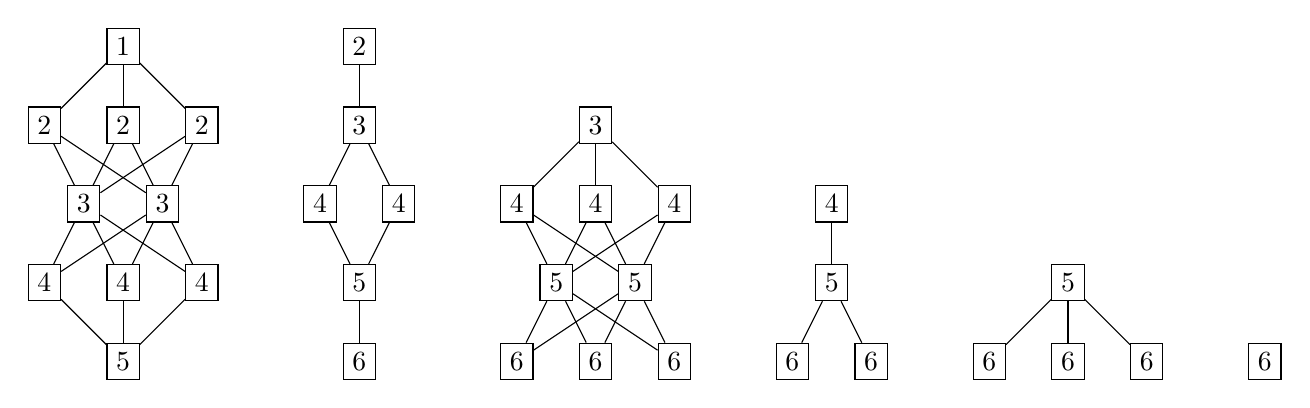
\begin{tikzpicture}
 
 \node at (3,0) [rectangle,draw] (1) {$1$};
 \node at (2,-1) [rectangle,draw] (2) {$2$};
 \node at (3,-1) [rectangle,draw] (3) {$2$};
 \node at (4,-1) [rectangle,draw] (4) {$2$};
 \node at (2.5,-2) [rectangle,draw] (5) {$3$};
 \node at (3.5,-2) [rectangle,draw] (6) {$3$};
 \node at (2,-3) [rectangle,draw] (7) {$4$};
 \node at (3,-3) [rectangle,draw] (8) {$4$};
 \node at (4,-3) [rectangle,draw] (9) {$4$};
 \node at (3,-4) [rectangle,draw] (10) {$5$};
 
 
 \draw (1)--(2);
 \draw (1)--(3);
  \draw (1)--(4);
 \draw (2)--(5);  
  \draw (2)--(6);
   \draw (3)--(5);
    \draw (3)--(6);
    
     \draw (4)--(5);
      \draw (4)--(6);
       \draw (5)--(7);
        \draw (5)--(8);
         \draw (5)--(9);
          \draw (6)--(7);
           \draw (6)--(8);
            \draw (6)--(9);
             \draw (7)--(10);
              \draw (8)--(10);
               \draw (9)--(10);
\begin{scope}[xshift={3cm}]
 \node at (3,0) [rectangle,draw] (1) {$2$};
  \node at (3,-1) [rectangle,draw] (3) {$3$};
  \node at (2.5,-2) [rectangle,draw] (5) {$4$};
 \node at (3.5,-2) [rectangle,draw] (6) {$4$};
  \node at (3,-3) [rectangle,draw] (8) {$5$};
 \node at (3,-4) [rectangle,draw] (9) {$6$};
 \draw (1)--(3);\draw (3)--(5);\draw (3)--(6);\draw (5)--(8);\draw (6)--(8);\draw (8)--(9);
   \end{scope}
   
   
  \begin{scope}[xshift={6cm}]

 
 \node at (3,-1) [rectangle,draw] (6) {$3$};
 \node at (2,-2) [rectangle,draw] (7) {$4$};
 \node at (3,-2) [rectangle,draw] (8) {$4$};
 \node at (4,-2) [rectangle,draw] (9) {$4$};
 \node at (3.5,-3) [rectangle,draw] (10) {$5$};
  \node at (2.5,-3) [rectangle,draw] (11) {$5$};
  \node at (3,-4) [rectangle,draw] (12) {$6$};
   \node at (2,-4) [rectangle,draw] (13) {$6$};
    \node at (4,-4) [rectangle,draw] (14) {$6$};
    
\draw (6)--(7);\draw (7)--(11);\draw (11)--(12);
  \draw (6)--(8);\draw (8)--(11);\draw (11)--(13);
  \draw (6)--(9);\draw (9)--(11);\draw (11)--(14);
    \draw (7)--(10);\draw (10)--(12);
      \draw (8)--(10);\draw (10)--(13);
         \draw (9)--(10);\draw (10)--(14);
  \end{scope}
  
   \begin{scope}[xshift={9cm}]

 \node at (3,-2) [rectangle,draw] (7) {$4$};
   \node at (3,-3) [rectangle,draw] (11) {$5$};
  \node at (2.5,-4) [rectangle,draw] (12) {$6$};
   \node at (3.5,-4) [rectangle,draw] (13) {$6$};
          \draw (7)--(11);\draw (11)--(12);
           \draw (11)--(13);
  \end{scope}
  \begin{scope}[xshift={14cm}]


   \node at (3.5,-4) [rectangle,draw] (13) {$6$};
       
  \end{scope}
  \begin{scope}[xshift={12cm}]

 
   \node at (3,-3) [rectangle,draw] (11) {$5$};
  \node at (2,-4) [rectangle,draw] (12) {$6$};
   \node at (3,-4) [rectangle,draw] (13) {$6$};
   \node at (4,-4) [rectangle,draw] (14) {$6$};
          \draw (11)--(14);\draw (11)--(12);
           \draw (11)--(13);
  \end{scope}
\end{tikzpicture}

\end{minipage}
\vspace{1cm}\\
It follows that $\gldim B=2=\domdim B$, so it is a Auslander algebra. Now we consider the following algebra $B'$ whose projective objects are



\begin{minipage}{.5\textwidth}
\centering

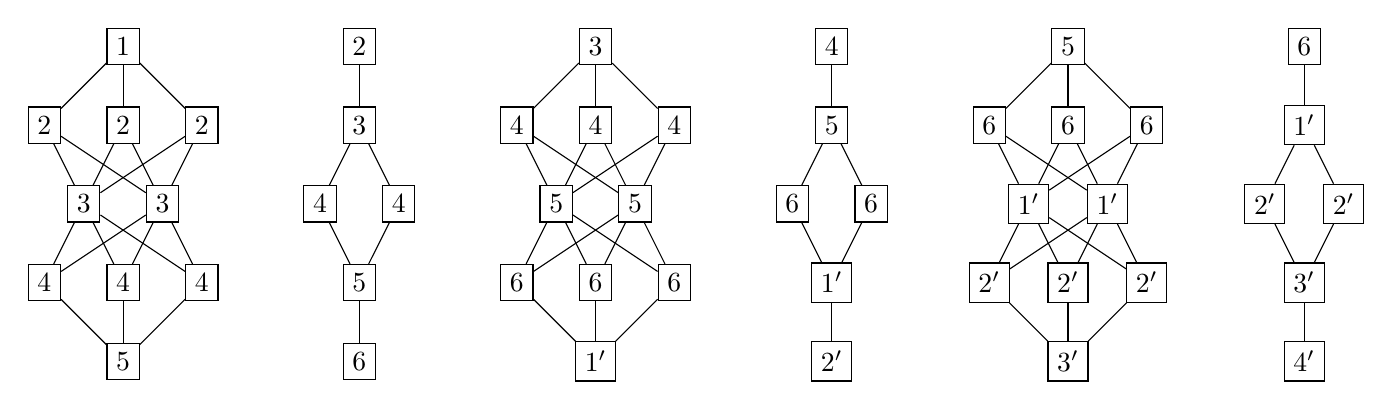
\begin{tikzpicture}
 
 \node at (3,0) [rectangle,draw] (1) {$1$};
 \node at (2,-1) [rectangle,draw] (2) {$2$};
 \node at (3,-1) [rectangle,draw] (3) {$2$};
 \node at (4,-1) [rectangle,draw] (4) {$2$};
 \node at (2.5,-2) [rectangle,draw] (5) {$3$};
 \node at (3.5,-2) [rectangle,draw] (6) {$3$};
 \node at (2,-3) [rectangle,draw] (7) {$4$};
 \node at (3,-3) [rectangle,draw] (8) {$4$};
 \node at (4,-3) [rectangle,draw] (9) {$4$};
 \node at (3,-4) [rectangle,draw] (10) {$5$};
 
 
 \draw (1)--(2); \draw (1)--(3);  \draw (1)--(4);
 \draw (2)--(5);    \draw (2)--(6);   \draw (3)--(5);
    \draw (3)--(6);\draw (4)--(5);\draw (4)--(6);
\draw (5)--(7); \draw (5)--(8);  \draw (5)--(9);
 \draw (6)--(7);\draw (6)--(8);\draw (6)--(9);
 \draw (7)--(10); \draw (8)--(10); \draw (9)--(10);
 
\begin{scope}[xshift={3cm}]
 \node at (3,0) [rectangle,draw] (1) {$2$};
  \node at (3,-1) [rectangle,draw] (3) {$3$};
  \node at (2.5,-2) [rectangle,draw] (5) {$4$};
 \node at (3.5,-2) [rectangle,draw] (6) {$4$};
  \node at (3,-3) [rectangle,draw] (8) {$5$};
 \node at (3,-4) [rectangle,draw] (9) {$6$};
 \draw (1)--(3);\draw (3)--(5);\draw (3)--(6);\draw (5)--(8);\draw (6)--(8);\draw (8)--(9);
   \end{scope}
   
   
  \begin{scope}[xshift={6cm}]

 
 \node at (3,0) [rectangle,draw] (6) {$3$};
 \node at (2,-1) [rectangle,draw] (7) {$4$};
 \node at (3,-1) [rectangle,draw] (8) {$4$};
 \node at (4,-1) [rectangle,draw] (9) {$4$};
 \node at (3.5,-2) [rectangle,draw] (10) {$5$};
  \node at (2.5,-2) [rectangle,draw] (11) {$5$};
  \node at (3,-3) [rectangle,draw] (12) {$6$};
   \node at (2,-3) [rectangle,draw] (13) {$6$};
    \node at (4,-3) [rectangle,draw] (14) {$6$};
    \node at (3,-4) [rectangle,draw] (15) {$1'$};
    
\draw (6)--(7);\draw (7)--(11);\draw (11)--(12);
  \draw (6)--(8);\draw (8)--(11);\draw (11)--(13);
  \draw (6)--(9);\draw (9)--(11);\draw (11)--(14);
    \draw (7)--(10);\draw (10)--(12);\draw (12)--(15);
      \draw (8)--(10);\draw (10)--(13);\draw (13)--(15);
         \draw (9)--(10);\draw (10)--(14);\draw (14)--(15);
  \end{scope}
  
   \begin{scope}[xshift={9cm}]

 \node at (3,0) [rectangle,draw] (7) {$4$};
   \node at (3,-1) [rectangle,draw] (11) {$5$};
  \node at (2.5,-2) [rectangle,draw] (12) {$6$};
   \node at (3.5,-2) [rectangle,draw] (13) {$6$};
    \node at (3,-3) [rectangle,draw] (1) {$1'$};
   \node at (3,-4) [rectangle,draw] (2) {$2'$};
          \draw (7)--(11);\draw (11)--(12);
           \draw (11)--(13);\draw (12)--(1);
           \draw (13)--(1);\draw (1)--(2);
  \end{scope}
  \begin{scope}[xshift={15cm}]


  \node at (3,0) [rectangle,draw] (1) {$6$};
  \node at (3,-1) [rectangle,draw] (3) {$1'$};
  \node at (2.5,-2) [rectangle,draw] (5) {$2'$};
 \node at (3.5,-2) [rectangle,draw] (6) {$2'$};
  \node at (3,-3) [rectangle,draw] (8) {$3'$};
 \node at (3,-4) [rectangle,draw] (9) {$4'$};
 \draw (1)--(3);\draw (3)--(5);\draw (3)--(6);\draw (5)--(8);\draw (6)--(8);\draw (8)--(9);
       
  \end{scope}
  \begin{scope}[xshift={12cm}]

 \node at (3,0) [rectangle,draw] (1) {$5$};
 \node at (2,-1) [rectangle,draw] (2) {$6$};
 \node at (3,-1) [rectangle,draw] (3) {$6$};
 \node at (4,-1) [rectangle,draw] (4) {$6$};
 \node at (2.5,-2) [rectangle,draw] (5) {$1'$};
 \node at (3.5,-2) [rectangle,draw] (6) {$1'$};
 \node at (2,-3) [rectangle,draw] (7) {$2'$};
 \node at (3,-3) [rectangle,draw] (8) {$2'$};
 \node at (4,-3) [rectangle,draw] (9) {$2'$};
 \node at (3,-4) [rectangle,draw] (10) {$3'$};
 
 
 \draw (1)--(2); \draw (1)--(3);  \draw (1)--(4);
 \draw (2)--(5);    \draw (2)--(6);   \draw (3)--(5);
    \draw (3)--(6);\draw (4)--(5);\draw (4)--(6);
\draw (5)--(7); \draw (5)--(8);  \draw (5)--(9);
 \draw (6)--(7);\draw (6)--(8);\draw (6)--(9);
 \draw (7)--(10); \draw (8)--(10); \draw (9)--(10);
  \end{scope}
\end{tikzpicture}

\end{minipage}



\begin{minipage}{.5\textwidth}
\centering

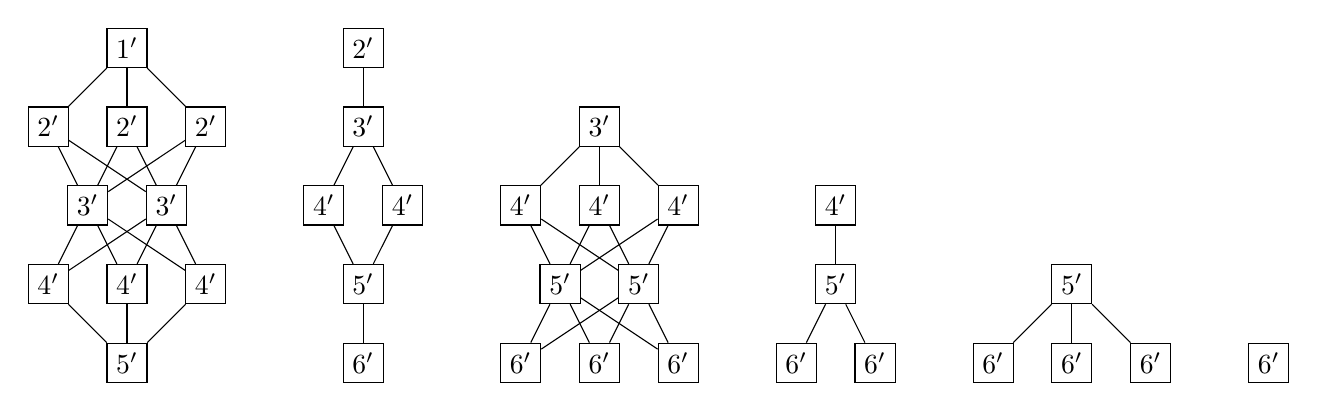
\begin{tikzpicture}
 
 \node at (3,0) [rectangle,draw] (1) {$1'$};
 \node at (2,-1) [rectangle,draw] (2) {$2'$};
 \node at (3,-1) [rectangle,draw] (3) {$2'$};
 \node at (4,-1) [rectangle,draw] (4) {$2'$};
 \node at (2.5,-2) [rectangle,draw] (5) {$3'$};
 \node at (3.5,-2) [rectangle,draw] (6) {$3'$};
 \node at (2,-3) [rectangle,draw] (7) {$4'$};
 \node at (3,-3) [rectangle,draw] (8) {$4'$};
 \node at (4,-3) [rectangle,draw] (9) {$4'$};
 \node at (3,-4) [rectangle,draw] (10) {$5'$};
 
 
 \draw (1)--(2);
 \draw (1)--(3);
  \draw (1)--(4);
 \draw (2)--(5);  
  \draw (2)--(6);
   \draw (3)--(5);
    \draw (3)--(6);
    
     \draw (4)--(5);
      \draw (4)--(6);
       \draw (5)--(7);
        \draw (5)--(8);
         \draw (5)--(9);
          \draw (6)--(7);
           \draw (6)--(8);
            \draw (6)--(9);
             \draw (7)--(10);
              \draw (8)--(10);
               \draw (9)--(10);
\begin{scope}[xshift={3cm}]
 \node at (3,0) [rectangle,draw] (1) {$2'$};
  \node at (3,-1) [rectangle,draw] (3) {$3'$};
  \node at (2.5,-2) [rectangle,draw] (5) {$4'$};
 \node at (3.5,-2) [rectangle,draw] (6) {$4'$};
  \node at (3,-3) [rectangle,draw] (8) {$5'$};
 \node at (3,-4) [rectangle,draw] (9) {$6'$};
 \draw (1)--(3);\draw (3)--(5);\draw (3)--(6);\draw (5)--(8);\draw (6)--(8);\draw (8)--(9);
   \end{scope}
   
   
  \begin{scope}[xshift={6cm}]

 
 \node at (3,-1) [rectangle,draw] (6) {$3'$};
 \node at (2,-2) [rectangle,draw] (7) {$4'$};
 \node at (3,-2) [rectangle,draw] (8) {$4'$};
 \node at (4,-2) [rectangle,draw] (9) {$4'$};
 \node at (3.5,-3) [rectangle,draw] (10) {$5'$};
  \node at (2.5,-3) [rectangle,draw] (11) {$5'$};
  \node at (3,-4) [rectangle,draw] (12) {$6'$};
   \node at (2,-4) [rectangle,draw] (13) {$6'$};
    \node at (4,-4) [rectangle,draw] (14) {$6'$};
    
\draw (6)--(7);\draw (7)--(11);\draw (11)--(12);
  \draw (6)--(8);\draw (8)--(11);\draw (11)--(13);
  \draw (6)--(9);\draw (9)--(11);\draw (11)--(14);
    \draw (7)--(10);\draw (10)--(12);
      \draw (8)--(10);\draw (10)--(13);
         \draw (9)--(10);\draw (10)--(14);
  \end{scope}
  
   \begin{scope}[xshift={9cm}]

 \node at (3,-2) [rectangle,draw] (7) {$4'$};
   \node at (3,-3) [rectangle,draw] (11) {$5'$};
  \node at (2.5,-4) [rectangle,draw] (12) {$6'$};
   \node at (3.5,-4) [rectangle,draw] (13) {$6'$};
          \draw (7)--(11);\draw (11)--(12);
           \draw (11)--(13);
  \end{scope}
  \begin{scope}[xshift={14cm}]


   \node at (3.5,-4) [rectangle,draw] (13) {$6'$};
       
  \end{scope}
  \begin{scope}[xshift={12cm}]

 
   \node at (3,-3) [rectangle,draw] (11) {$5'$};
  \node at (2,-4) [rectangle,draw] (12) {$6'$};
   \node at (3,-4) [rectangle,draw] (13) {$6'$};
   \node at (4,-4) [rectangle,draw] (14) {$6'$};
          \draw (11)--(14);\draw (11)--(12);
           \draw (11)--(13);
  \end{scope}
\end{tikzpicture}

\end{minipage}

One can verify that $\gldim B'=5=\domdim B'$. Moreover, by choice of simple modules, it is duplicated algebra of $B$. We constructed this algebra by looking not Auslander-Reiten quiver of Dynkin quiver $G_2$ but from the following quiver which presents all irreducible maps of $\modd G_2$.


\begin{align*}
\xymatrixcolsep{4mm}
\xymatrix{
   P_1\ar[rd] && P_1/P_2\ar[rd] && I_1\ar[rd] && P_1[1]\ar[rd] && P_1/P_2[1]\ar[rd]&&I_1[1]\ar[rd]&\\
   P_1\ar[r]& P_2 \ar[r]\ar[ru]\ar[rd]& P_1/P_2\ar[r]&Y\ar[r]\ar[ru]\ar[rd]&I_1\ar[r]&I_2\ar[ru]\ar[r]\ar[rd]& P_1[1]\ar[r]&P_2[1]\ar[ru]\ar[r]\ar[rd]&P_1/P_2[1]\ar[r]&Y[1]\ar[ru]\ar[r]\ar[rd]&I_2[1]\ar[r]&I_1[1]&\\
   P_1\ar[ru] && P_1/P_2\ar[ru] && I_1\ar[ru] &&P_1[1]\ar[ru]&&P_1/P_2[1]\ar[ru]&&I_2[1]\ar[ru]}
\end{align*}
where $P_1, P_2$ are the modules $0\rightarrow F$, $G\rightarrow F$ where $[G:F]$ is degree three extension of field $F$. Moreover, one can verify that similar constructions work for non simply laced Dynkin quivers. 
We wonder whether there exists higher analogues of K-species studied in \cite{dlab1976indecomposable} from the higher homological algebra point of view.




%\bibliographystyle{alpha}
%\bibliography{derivedcat}

\bibliographystyle{alpha}
\begin{thebibliography}{99}
\bibitem[ABST06]{ASSEM2006548}
I.~Assem, T.~Brüstle, R.~Schiffler, and G.~Todorov.
\newblock Cluster categories and duplicated algebras.
\newblock {\em Journal of Algebra}, 305(1):548--561, 2006.

\bibitem[ABST08]{ASSEM2008884}
I.~Assem, T.~Brüstle, R.~Schiffler, and G.~Todorov.
\newblock m-cluster categories and m-replicated algebras.
\newblock {\em Journal of Pure and Applied Algebra}, 212(4):884--901, 2008.

\bibitem[ARS97]{auslander1997representation}
Maurice Auslander, Idun Reiten, and Sverre~O Smalo.
\newblock {\em Representation theory of Artin algebras}, volume~36.
\newblock Cambridge university press, 1997.

\bibitem[BMRRT06]{buan2006tilting}
Aslak~Bakke Buan, Bethany~Rose Marsh, Markus Reineke, Idun Reiten, and Gordana
  Todorov.
\newblock Tilting theory and cluster combinatorics.
\newblock {\em Advances in mathematics}, 204(2):572--618, 2006.

\bibitem[DI20]{darpo2020d}
Erik Darp{\"o} and Osamu Iyama.
\newblock d-representation-finite self-injective algebras.
\newblock {\em Advances in Mathematics}, 362:106932, 2020.

\bibitem[DR76]{dlab1976indecomposable}
Vlastimil Dlab and Claus~Michael Ringel.
\newblock {\em Indecomposable representations of graphs and algebras}.
\newblock Number 6-173. American Mathematical Soc., 1976.

\bibitem[GKO13]{geiss2013n}
Christof Geiss, Bernhard Keller, and Steffen Oppermann.
\newblock n-angulated categories.
\newblock {\em Journal f{\"u}r die reine und angewandte Mathematik (Crelles
  Journal)}, 2013(675):101--120, 2013.

\bibitem[Hap88]{happel1988triangulated}
Dieter Happel.
\newblock {\em Triangulated categories in the representation of finite
  dimensional algebras}, volume 119.
\newblock Cambridge University Press, 1988.

\bibitem[HI11]{herschend2011fractionally}
Martin Herschend and Osamu Iyama.
\newblock n-representation-finite algebras and twisted fractionally calabi-yau
  algebras.
\newblock {\em Bulletin of the London Mathematical Society}, 43(3):449--466,
  2011.

\bibitem[HIO14]{herschend2014iyamaopperman}
Martin Herschend, Osamu Iyama, and Steffen Oppermann.
\newblock n-representation infinite algebras.
\newblock {\em Advances in Mathematics}, 252:292--342, 2014.

\bibitem[HJS22]{haugland2022role}
Johanne Haugland, Karin~M Jacobsen, and Sibylle Schroll.
\newblock The role of gentle algebras in higher homological algebra.
\newblock In {\em Forum Mathematicum}, volume~34, pages 1255--1275. De Gruyter,
  2022.

\bibitem[Iya07]{iyama2007auslandercorrespondence}
Osamu Iyama.
\newblock Auslander correspondence.
\newblock {\em Advances in Mathematics}, 210(1):51--82, 2007.

\bibitem[Iya08]{iyama2008auslanderreitenrevisited}
Osamu Iyama.
\newblock Auslander-reiten theory revisited.
\newblock {\em arXiv preprint arXiv:0803.2841}, 2008.

\bibitem[Iya11]{iyama2011clusterMAINpaper}
Osamu Iyama.
\newblock Cluster tilting for higher auslander algebras.
\newblock {\em Advances in Mathematics}, 226(1):1--61, 2011.

\bibitem[Jas16]{jasso2016n}
Gustavo Jasso.
\newblock n-abelian and n-exact categories.
\newblock {\em Mathematische Zeitschrift}, 283:703--759, 2016.

\bibitem[JKPK19]{julianNakayama}
Gustavo Jasso, Julian K{\"u}lshammer, Chrysostomos Psaroudakis, and Sondre
  Kvamme.
\newblock Higher nakayama algebras i: construction.
\newblock {\em Advances in Mathematics}, 351:1139--1200, 2019.

\bibitem[Kel05]{keller2005triangulated}
Bernhard Keller.
\newblock On triangulated orbit categories.
\newblock {\em Documenta Mathematica}, 10:551--581, 2005.

\bibitem[OT12]{oppermann2012higher}
Steffen Oppermann and Hugh~R Thomas.
\newblock Higher-dimensional cluster combinatorics and representation theory.
\newblock {\em Journal of the European Mathematical Society}, 14(6):1679--1737,
  2012.

\bibitem[Rei10]{reiten2010cluster}
Idun Reiten.
\newblock Cluster categories.
\newblock In {\em Proceedings of the International Congress of Mathematicians
  2010 (ICM 2010) (In 4 Volumes) Vol. I: Plenary Lectures and Ceremonies Vols.
  II--IV: Invited Lectures}, pages 558--594. World Scientific, 2010.

\bibitem[Rin22]{ringel2022linear}
Claus~Michael Ringel.
\newblock Linear nakayama algebras which are higher auslander algebras.
\newblock {\em Communications in Algebra}, 50(11):4842--4881, 2022.

\bibitem[Sen20]{sen2020nakayama}
Emre Sen.
\newblock Nakayama algebras which are higher auslander algebras.
\newblock {\em arXiv preprint arXiv:2009.03383}, 2020.

\bibitem[STZ]{senDefectlinear}
Emre Sen, Gordana Todorov, and Shijie Zhu.
\newblock Defect invariant linear nakayama algebras.
\newblock {\em in preparation}.

\bibitem[Vas19]{vaso2019n}
Laertis Vaso.
\newblock n-cluster tilting subcategories of representation-directed algebras.
\newblock {\em Journal of Pure and Applied Algebra}, 223(5):2101--2122, 2019.

\end{thebibliography}


\end{document}






\section{deleted part}

\begin{align*}
\xymatrixcolsep{1mm}
\xymatrix{
1\ar[rr]&&2\ar[rr]&&3&&&&&&&&\\
1\ar[rr]&&2&&&&&&&&&\\
1&&&&&&&&&&\\
&&1'\ar[rr]&&2'\ar[rr]\ar[lllluu]&&3'\ar[lllluu]&&&&&&&\\
&&1'\ar[rr]&&2'\ar[lllluu]&&&&&&&&\\
&&1'&&&&&&&&&\\
&&&&1'\ar[rr]&&2'\ar[rr]&&3'&&&&&&&\\
&&&&1'\ar[rr]&&2'&&&&&&&&\\
&&&&1'&&&&&&&&&\\
&&&&&1'\ar[rr]&&2'\ar[rr]&&3'&&&&&\\
&&&&&1'\ar[rr]&&2'&&&&&&\\
&&&&&1'&&&&&&&\\
&&&&&&&1'\ar[rr]&&2'\ar[rr]&&3'&&&&&\\
&&&&&&&1'\ar[rr]&&2'&&&&&&\\
&&&&&&&1'&&&&&&&\\
}
\end{align*}
